
% Default to the notebook output style

    


% Inherit from the specified cell style.




    
\documentclass[11pt]{article}

    
    
    \usepackage[T1]{fontenc}
    % Nicer default font (+ math font) than Computer Modern for most use cases
    \usepackage{mathpazo}

    % Basic figure setup, for now with no caption control since it's done
    % automatically by Pandoc (which extracts ![](path) syntax from Markdown).
    \usepackage{graphicx}
    % We will generate all images so they have a width \maxwidth. This means
    % that they will get their normal width if they fit onto the page, but
    % are scaled down if they would overflow the margins.
    \makeatletter
    \def\maxwidth{\ifdim\Gin@nat@width>\linewidth\linewidth
    \else\Gin@nat@width\fi}
    \makeatother
    \let\Oldincludegraphics\includegraphics
    % Set max figure width to be 80% of text width, for now hardcoded.
    \renewcommand{\includegraphics}[1]{\Oldincludegraphics[width=.8\maxwidth]{#1}}
    % Ensure that by default, figures have no caption (until we provide a
    % proper Figure object with a Caption API and a way to capture that
    % in the conversion process - todo).
    \usepackage{caption}
    % \DeclareCaptionLabelFormat{nolabel}{}
    % \captionsetup{labelformat=nolabel}

    \usepackage{adjustbox} % Used to constrain images to a maximum size 
    \usepackage{xcolor} % Allow colors to be defined
    \usepackage{enumerate} % Needed for markdown enumerations to work
    \usepackage{geometry} % Used to adjust the document margins
    \usepackage{amsmath} % Equations
    \usepackage{amssymb} % Equations
    \usepackage{textcomp} % defines textquotesingle
    % Hack from http://tex.stackexchange.com/a/47451/13684:
    \AtBeginDocument{%
        \def\PYZsq{\textquotesingle}% Upright quotes in Pygmentized code
    }
    \usepackage{upquote} % Upright quotes for verbatim code
    \usepackage{eurosym} % defines \euro
    \usepackage[mathletters]{ucs} % Extended unicode (utf-8) support
    \usepackage[utf8x]{inputenc} % Allow utf-8 characters in the tex document
    \usepackage{fancyvrb} % verbatim replacement that allows latex
    \usepackage{grffile} % extends the file name processing of package graphics 
                         % to support a larger range 
    % The hyperref package gives us a pdf with properly built
    % internal navigation ('pdf bookmarks' for the table of contents,
    % internal cross-reference links, web links for URLs, etc.)
    \usepackage{hyperref}
    \usepackage{longtable} % longtable support required by pandoc >1.10
    \usepackage{booktabs}  % table support for pandoc > 1.12.2
    \usepackage[inline]{enumitem} % IRkernel/repr support (it uses the enumerate* environment)
    \usepackage[normalem]{ulem} % ulem is needed to support strikethroughs (\sout)
                                % normalem makes italics be italics, not underlines
    \usepackage{mathrsfs}
    

    
    
    % Colors for the hyperref package
    \definecolor{urlcolor}{rgb}{0,.145,.698}
    \definecolor{linkcolor}{rgb}{.71,0.21,0.01}
    \definecolor{citecolor}{rgb}{.12,.54,.11}

    % ANSI colors
    \definecolor{ansi-black}{HTML}{3E424D}
    \definecolor{ansi-black-intense}{HTML}{282C36}
    \definecolor{ansi-red}{HTML}{E75C58}
    \definecolor{ansi-red-intense}{HTML}{B22B31}
    \definecolor{ansi-green}{HTML}{00A250}
    \definecolor{ansi-green-intense}{HTML}{007427}
    \definecolor{ansi-yellow}{HTML}{DDB62B}
    \definecolor{ansi-yellow-intense}{HTML}{B27D12}
    \definecolor{ansi-blue}{HTML}{208FFB}
    \definecolor{ansi-blue-intense}{HTML}{0065CA}
    \definecolor{ansi-magenta}{HTML}{D160C4}
    \definecolor{ansi-magenta-intense}{HTML}{A03196}
    \definecolor{ansi-cyan}{HTML}{60C6C8}
    \definecolor{ansi-cyan-intense}{HTML}{258F8F}
    \definecolor{ansi-white}{HTML}{C5C1B4}
    \definecolor{ansi-white-intense}{HTML}{A1A6B2}
    \definecolor{ansi-default-inverse-fg}{HTML}{FFFFFF}
    \definecolor{ansi-default-inverse-bg}{HTML}{000000}

    % commands and environments needed by pandoc snippets
    % extracted from the output of `pandoc -s`
    \providecommand{\tightlist}{%
      \setlength{\itemsep}{0pt}\setlength{\parskip}{0pt}}
    \DefineVerbatimEnvironment{Highlighting}{Verbatim}{commandchars=\\\{\}}
    % Add ',fontsize=\small' for more characters per line
    \newenvironment{Shaded}{}{}
    \newcommand{\KeywordTok}[1]{\textcolor[rgb]{0.00,0.44,0.13}{\textbf{{#1}}}}
    \newcommand{\DataTypeTok}[1]{\textcolor[rgb]{0.56,0.13,0.00}{{#1}}}
    \newcommand{\DecValTok}[1]{\textcolor[rgb]{0.25,0.63,0.44}{{#1}}}
    \newcommand{\BaseNTok}[1]{\textcolor[rgb]{0.25,0.63,0.44}{{#1}}}
    \newcommand{\FloatTok}[1]{\textcolor[rgb]{0.25,0.63,0.44}{{#1}}}
    \newcommand{\CharTok}[1]{\textcolor[rgb]{0.25,0.44,0.63}{{#1}}}
    \newcommand{\StringTok}[1]{\textcolor[rgb]{0.25,0.44,0.63}{{#1}}}
    \newcommand{\CommentTok}[1]{\textcolor[rgb]{0.38,0.63,0.69}{\textit{{#1}}}}
    \newcommand{\OtherTok}[1]{\textcolor[rgb]{0.00,0.44,0.13}{{#1}}}
    \newcommand{\AlertTok}[1]{\textcolor[rgb]{1.00,0.00,0.00}{\textbf{{#1}}}}
    \newcommand{\FunctionTok}[1]{\textcolor[rgb]{0.02,0.16,0.49}{{#1}}}
    \newcommand{\RegionMarkerTok}[1]{{#1}}
    \newcommand{\ErrorTok}[1]{\textcolor[rgb]{1.00,0.00,0.00}{\textbf{{#1}}}}
    \newcommand{\NormalTok}[1]{{#1}}
    
    % Additional commands for more recent versions of Pandoc
    \newcommand{\ConstantTok}[1]{\textcolor[rgb]{0.53,0.00,0.00}{{#1}}}
    \newcommand{\SpecialCharTok}[1]{\textcolor[rgb]{0.25,0.44,0.63}{{#1}}}
    \newcommand{\VerbatimStringTok}[1]{\textcolor[rgb]{0.25,0.44,0.63}{{#1}}}
    \newcommand{\SpecialStringTok}[1]{\textcolor[rgb]{0.73,0.40,0.53}{{#1}}}
    \newcommand{\ImportTok}[1]{{#1}}
    \newcommand{\DocumentationTok}[1]{\textcolor[rgb]{0.73,0.13,0.13}{\textit{{#1}}}}
    \newcommand{\AnnotationTok}[1]{\textcolor[rgb]{0.38,0.63,0.69}{\textbf{\textit{{#1}}}}}
    \newcommand{\CommentVarTok}[1]{\textcolor[rgb]{0.38,0.63,0.69}{\textbf{\textit{{#1}}}}}
    \newcommand{\VariableTok}[1]{\textcolor[rgb]{0.10,0.09,0.49}{{#1}}}
    \newcommand{\ControlFlowTok}[1]{\textcolor[rgb]{0.00,0.44,0.13}{\textbf{{#1}}}}
    \newcommand{\OperatorTok}[1]{\textcolor[rgb]{0.40,0.40,0.40}{{#1}}}
    \newcommand{\BuiltInTok}[1]{{#1}}
    \newcommand{\ExtensionTok}[1]{{#1}}
    \newcommand{\PreprocessorTok}[1]{\textcolor[rgb]{0.74,0.48,0.00}{{#1}}}
    \newcommand{\AttributeTok}[1]{\textcolor[rgb]{0.49,0.56,0.16}{{#1}}}
    \newcommand{\InformationTok}[1]{\textcolor[rgb]{0.38,0.63,0.69}{\textbf{\textit{{#1}}}}}
    \newcommand{\WarningTok}[1]{\textcolor[rgb]{0.38,0.63,0.69}{\textbf{\textit{{#1}}}}}
    
    
    % Define a nice break command that doesn't care if a line doesn't already
    % exist.
    \def\br{\hspace*{\fill} \\* }
    % Math Jax compatibility definitions
    \def\gt{>}
    \def\lt{<}
    \let\Oldtex\TeX
    \let\Oldlatex\LaTeX
    \renewcommand{\TeX}{\textrm{\Oldtex}}
    \renewcommand{\LaTeX}{\textrm{\Oldlatex}}
    % Document parameters
    % Document title
    \title{solution\_of\_team13\_problem}
    
    
    
    
    

    % Pygments definitions
    
\makeatletter
\def\PY@reset{\let\PY@it=\relax \let\PY@bf=\relax%
    \let\PY@ul=\relax \let\PY@tc=\relax%
    \let\PY@bc=\relax \let\PY@ff=\relax}
\def\PY@tok#1{\csname PY@tok@#1\endcsname}
\def\PY@toks#1+{\ifx\relax#1\empty\else%
    \PY@tok{#1}\expandafter\PY@toks\fi}
\def\PY@do#1{\PY@bc{\PY@tc{\PY@ul{%
    \PY@it{\PY@bf{\PY@ff{#1}}}}}}}
\def\PY#1#2{\PY@reset\PY@toks#1+\relax+\PY@do{#2}}

\expandafter\def\csname PY@tok@w\endcsname{\def\PY@tc##1{\textcolor[rgb]{0.73,0.73,0.73}{##1}}}
\expandafter\def\csname PY@tok@c\endcsname{\let\PY@it=\textit\def\PY@tc##1{\textcolor[rgb]{0.25,0.50,0.50}{##1}}}
\expandafter\def\csname PY@tok@cp\endcsname{\def\PY@tc##1{\textcolor[rgb]{0.74,0.48,0.00}{##1}}}
\expandafter\def\csname PY@tok@k\endcsname{\let\PY@bf=\textbf\def\PY@tc##1{\textcolor[rgb]{0.00,0.50,0.00}{##1}}}
\expandafter\def\csname PY@tok@kp\endcsname{\def\PY@tc##1{\textcolor[rgb]{0.00,0.50,0.00}{##1}}}
\expandafter\def\csname PY@tok@kt\endcsname{\def\PY@tc##1{\textcolor[rgb]{0.69,0.00,0.25}{##1}}}
\expandafter\def\csname PY@tok@o\endcsname{\def\PY@tc##1{\textcolor[rgb]{0.40,0.40,0.40}{##1}}}
\expandafter\def\csname PY@tok@ow\endcsname{\let\PY@bf=\textbf\def\PY@tc##1{\textcolor[rgb]{0.67,0.13,1.00}{##1}}}
\expandafter\def\csname PY@tok@nb\endcsname{\def\PY@tc##1{\textcolor[rgb]{0.00,0.50,0.00}{##1}}}
\expandafter\def\csname PY@tok@nf\endcsname{\def\PY@tc##1{\textcolor[rgb]{0.00,0.00,1.00}{##1}}}
\expandafter\def\csname PY@tok@nc\endcsname{\let\PY@bf=\textbf\def\PY@tc##1{\textcolor[rgb]{0.00,0.00,1.00}{##1}}}
\expandafter\def\csname PY@tok@nn\endcsname{\let\PY@bf=\textbf\def\PY@tc##1{\textcolor[rgb]{0.00,0.00,1.00}{##1}}}
\expandafter\def\csname PY@tok@ne\endcsname{\let\PY@bf=\textbf\def\PY@tc##1{\textcolor[rgb]{0.82,0.25,0.23}{##1}}}
\expandafter\def\csname PY@tok@nv\endcsname{\def\PY@tc##1{\textcolor[rgb]{0.10,0.09,0.49}{##1}}}
\expandafter\def\csname PY@tok@no\endcsname{\def\PY@tc##1{\textcolor[rgb]{0.53,0.00,0.00}{##1}}}
\expandafter\def\csname PY@tok@nl\endcsname{\def\PY@tc##1{\textcolor[rgb]{0.63,0.63,0.00}{##1}}}
\expandafter\def\csname PY@tok@ni\endcsname{\let\PY@bf=\textbf\def\PY@tc##1{\textcolor[rgb]{0.60,0.60,0.60}{##1}}}
\expandafter\def\csname PY@tok@na\endcsname{\def\PY@tc##1{\textcolor[rgb]{0.49,0.56,0.16}{##1}}}
\expandafter\def\csname PY@tok@nt\endcsname{\let\PY@bf=\textbf\def\PY@tc##1{\textcolor[rgb]{0.00,0.50,0.00}{##1}}}
\expandafter\def\csname PY@tok@nd\endcsname{\def\PY@tc##1{\textcolor[rgb]{0.67,0.13,1.00}{##1}}}
\expandafter\def\csname PY@tok@s\endcsname{\def\PY@tc##1{\textcolor[rgb]{0.73,0.13,0.13}{##1}}}
\expandafter\def\csname PY@tok@sd\endcsname{\let\PY@it=\textit\def\PY@tc##1{\textcolor[rgb]{0.73,0.13,0.13}{##1}}}
\expandafter\def\csname PY@tok@si\endcsname{\let\PY@bf=\textbf\def\PY@tc##1{\textcolor[rgb]{0.73,0.40,0.53}{##1}}}
\expandafter\def\csname PY@tok@se\endcsname{\let\PY@bf=\textbf\def\PY@tc##1{\textcolor[rgb]{0.73,0.40,0.13}{##1}}}
\expandafter\def\csname PY@tok@sr\endcsname{\def\PY@tc##1{\textcolor[rgb]{0.73,0.40,0.53}{##1}}}
\expandafter\def\csname PY@tok@ss\endcsname{\def\PY@tc##1{\textcolor[rgb]{0.10,0.09,0.49}{##1}}}
\expandafter\def\csname PY@tok@sx\endcsname{\def\PY@tc##1{\textcolor[rgb]{0.00,0.50,0.00}{##1}}}
\expandafter\def\csname PY@tok@m\endcsname{\def\PY@tc##1{\textcolor[rgb]{0.40,0.40,0.40}{##1}}}
\expandafter\def\csname PY@tok@gh\endcsname{\let\PY@bf=\textbf\def\PY@tc##1{\textcolor[rgb]{0.00,0.00,0.50}{##1}}}
\expandafter\def\csname PY@tok@gu\endcsname{\let\PY@bf=\textbf\def\PY@tc##1{\textcolor[rgb]{0.50,0.00,0.50}{##1}}}
\expandafter\def\csname PY@tok@gd\endcsname{\def\PY@tc##1{\textcolor[rgb]{0.63,0.00,0.00}{##1}}}
\expandafter\def\csname PY@tok@gi\endcsname{\def\PY@tc##1{\textcolor[rgb]{0.00,0.63,0.00}{##1}}}
\expandafter\def\csname PY@tok@gr\endcsname{\def\PY@tc##1{\textcolor[rgb]{1.00,0.00,0.00}{##1}}}
\expandafter\def\csname PY@tok@ge\endcsname{\let\PY@it=\textit}
\expandafter\def\csname PY@tok@gs\endcsname{\let\PY@bf=\textbf}
\expandafter\def\csname PY@tok@gp\endcsname{\let\PY@bf=\textbf\def\PY@tc##1{\textcolor[rgb]{0.00,0.00,0.50}{##1}}}
\expandafter\def\csname PY@tok@go\endcsname{\def\PY@tc##1{\textcolor[rgb]{0.53,0.53,0.53}{##1}}}
\expandafter\def\csname PY@tok@gt\endcsname{\def\PY@tc##1{\textcolor[rgb]{0.00,0.27,0.87}{##1}}}
\expandafter\def\csname PY@tok@err\endcsname{\def\PY@bc##1{\setlength{\fboxsep}{0pt}\fcolorbox[rgb]{1.00,0.00,0.00}{1,1,1}{\strut ##1}}}
\expandafter\def\csname PY@tok@kc\endcsname{\let\PY@bf=\textbf\def\PY@tc##1{\textcolor[rgb]{0.00,0.50,0.00}{##1}}}
\expandafter\def\csname PY@tok@kd\endcsname{\let\PY@bf=\textbf\def\PY@tc##1{\textcolor[rgb]{0.00,0.50,0.00}{##1}}}
\expandafter\def\csname PY@tok@kn\endcsname{\let\PY@bf=\textbf\def\PY@tc##1{\textcolor[rgb]{0.00,0.50,0.00}{##1}}}
\expandafter\def\csname PY@tok@kr\endcsname{\let\PY@bf=\textbf\def\PY@tc##1{\textcolor[rgb]{0.00,0.50,0.00}{##1}}}
\expandafter\def\csname PY@tok@bp\endcsname{\def\PY@tc##1{\textcolor[rgb]{0.00,0.50,0.00}{##1}}}
\expandafter\def\csname PY@tok@fm\endcsname{\def\PY@tc##1{\textcolor[rgb]{0.00,0.00,1.00}{##1}}}
\expandafter\def\csname PY@tok@vc\endcsname{\def\PY@tc##1{\textcolor[rgb]{0.10,0.09,0.49}{##1}}}
\expandafter\def\csname PY@tok@vg\endcsname{\def\PY@tc##1{\textcolor[rgb]{0.10,0.09,0.49}{##1}}}
\expandafter\def\csname PY@tok@vi\endcsname{\def\PY@tc##1{\textcolor[rgb]{0.10,0.09,0.49}{##1}}}
\expandafter\def\csname PY@tok@vm\endcsname{\def\PY@tc##1{\textcolor[rgb]{0.10,0.09,0.49}{##1}}}
\expandafter\def\csname PY@tok@sa\endcsname{\def\PY@tc##1{\textcolor[rgb]{0.73,0.13,0.13}{##1}}}
\expandafter\def\csname PY@tok@sb\endcsname{\def\PY@tc##1{\textcolor[rgb]{0.73,0.13,0.13}{##1}}}
\expandafter\def\csname PY@tok@sc\endcsname{\def\PY@tc##1{\textcolor[rgb]{0.73,0.13,0.13}{##1}}}
\expandafter\def\csname PY@tok@dl\endcsname{\def\PY@tc##1{\textcolor[rgb]{0.73,0.13,0.13}{##1}}}
\expandafter\def\csname PY@tok@s2\endcsname{\def\PY@tc##1{\textcolor[rgb]{0.73,0.13,0.13}{##1}}}
\expandafter\def\csname PY@tok@sh\endcsname{\def\PY@tc##1{\textcolor[rgb]{0.73,0.13,0.13}{##1}}}
\expandafter\def\csname PY@tok@s1\endcsname{\def\PY@tc##1{\textcolor[rgb]{0.73,0.13,0.13}{##1}}}
\expandafter\def\csname PY@tok@mb\endcsname{\def\PY@tc##1{\textcolor[rgb]{0.40,0.40,0.40}{##1}}}
\expandafter\def\csname PY@tok@mf\endcsname{\def\PY@tc##1{\textcolor[rgb]{0.40,0.40,0.40}{##1}}}
\expandafter\def\csname PY@tok@mh\endcsname{\def\PY@tc##1{\textcolor[rgb]{0.40,0.40,0.40}{##1}}}
\expandafter\def\csname PY@tok@mi\endcsname{\def\PY@tc##1{\textcolor[rgb]{0.40,0.40,0.40}{##1}}}
\expandafter\def\csname PY@tok@il\endcsname{\def\PY@tc##1{\textcolor[rgb]{0.40,0.40,0.40}{##1}}}
\expandafter\def\csname PY@tok@mo\endcsname{\def\PY@tc##1{\textcolor[rgb]{0.40,0.40,0.40}{##1}}}
\expandafter\def\csname PY@tok@ch\endcsname{\let\PY@it=\textit\def\PY@tc##1{\textcolor[rgb]{0.25,0.50,0.50}{##1}}}
\expandafter\def\csname PY@tok@cm\endcsname{\let\PY@it=\textit\def\PY@tc##1{\textcolor[rgb]{0.25,0.50,0.50}{##1}}}
\expandafter\def\csname PY@tok@cpf\endcsname{\let\PY@it=\textit\def\PY@tc##1{\textcolor[rgb]{0.25,0.50,0.50}{##1}}}
\expandafter\def\csname PY@tok@c1\endcsname{\let\PY@it=\textit\def\PY@tc##1{\textcolor[rgb]{0.25,0.50,0.50}{##1}}}
\expandafter\def\csname PY@tok@cs\endcsname{\let\PY@it=\textit\def\PY@tc##1{\textcolor[rgb]{0.25,0.50,0.50}{##1}}}

\def\PYZbs{\char`\\}
\def\PYZus{\char`\_}
\def\PYZob{\char`\{}
\def\PYZcb{\char`\}}
\def\PYZca{\char`\^}
\def\PYZam{\char`\&}
\def\PYZlt{\char`\<}
\def\PYZgt{\char`\>}
\def\PYZsh{\char`\#}
\def\PYZpc{\char`\%}
\def\PYZdl{\char`\$}
\def\PYZhy{\char`\-}
\def\PYZsq{\char`\'}
\def\PYZdq{\char`\"}
\def\PYZti{\char`\~}
% for compatibility with earlier versions
\def\PYZat{@}
\def\PYZlb{[}
\def\PYZrb{]}
\makeatother


    % Exact colors from NB
    \definecolor{incolor}{rgb}{0.0, 0.0, 0.5}
    \definecolor{outcolor}{rgb}{0.545, 0.0, 0.0}



    
    % Prevent overflowing lines due to hard-to-break entities
    \sloppy 
    % Setup hyperref package
    \hypersetup{
      breaklinks=true,  % so long urls are correctly broken across lines
      colorlinks=true,
      urlcolor=urlcolor,
      linkcolor=linkcolor,
      citecolor=citecolor,
      }
    % Slightly bigger margins than the latex defaults
    
    \geometry{verbose,tmargin=1in,bmargin=1in,lmargin=1in,rmargin=1in}
    
    \title{Solution of the TEAM 13 problem\\\small3d Non-Linear Magnetostatic Model}
    \author{Valentin Hanser, TU Wien}

    \begin{document}
    
    
    \maketitle
    
    

    
    \hypertarget{getting-started}{%
\section{Getting started}\label{getting-started}}

The script dependencies are: 
\begin{itemize}
	\item \href{https://ngsolve.org/downloads}{ngsolve} 
	\item \href{https://docs.scipy.org/doc/numpy/user/install.html}{numpy} 
	\item \href{https://scipy.org/install.html}{scipy} 
	\item \href{https://matplotlib.org/users/installing.html}{matplotlib} 
	\item the .vol file of the geometry \(\textit{./team13\_mesh.vol}\)
\end{itemize}

If the geometry file is erroneous, execute the python script
\(\texttt{./geometry.py}\), which generates the necessary
\(\texttt{.vol}\) file.

\begin{verbatim}
python3 geometry.py [-fullProblem True/False]
\end{verbatim}

    \hypertarget{problem-description}{%
\section{Problem Description}\label{problem-description}}

This script solves the T.E.A.M problem 13 (3-D Non-Linear Magnetostatic
Model). The problem description can be found under the
\href{https://www.compumag.org/wp/wp-content/uploads/2018/06/problem13.pdf}{link}.\\
The problem is based on the Maxwell equations with the corresponding
boundary conditions


\begin{align}
    \nabla \times \textbf{H} &= \textbf{J}, \qquad &&\textbf{H}\times\textbf{n} = \textbf{0}\\
    \nabla \cdot \textbf{B} &= 0,  &&\textbf{B}\cdot\textbf{n} = 0
\end{align}
for magnetostatic phenomena. The second equation allows the introduction
of a magnetic vector potential \(\textbf{A}\) as

     \begin{equation}
        \textbf{B} =  \nabla \times \textbf{A}.
    \end{equation}
For the weak formulation

    \begin{equation}
        \int_\Omega \frac{1}{\mu(|\textbf{B}|)}\nabla\times \textbf{A}\cdot \nabla\times\textbf{v}\; d\Omega = \int_{\Omega_c} \textbf{J}\cdot \textbf{v}\;d\Omega 
    \end{equation}
is used, which considers the non-linear material relationship


    \begin{equation}
        \textbf{H} =  \frac{1}{\mu(|\textbf{B}|)}\textbf{B}.
    \end{equation}
Wherein \(\textbf{A}\) and \(\textbf{v}\) are the trial and the test
function, \(\Omega\) is the domain of interest and \(\Omega_c\) is the
domain of the coil.\\
For a unique solution, an additional regularisation term with a small
\(\varepsilon > 0\) has been added:


    \begin{equation}
        \int_\Omega \frac{1}{\mu(|\textbf{B}|)}\nabla\times \textbf{A}\cdot \nabla\times\textbf{v}\; d\Omega + \int_\Omega\varepsilon\;\textbf{A}\cdot\textbf{v}\;d\Omega= \int_{\Omega_c} \textbf{J}\cdot \textbf{v}\;d\Omega              
    \end{equation}


The magnetic flux density of the solution is presented in Fig. 1.

\begin{figure}[h]
	\centering
	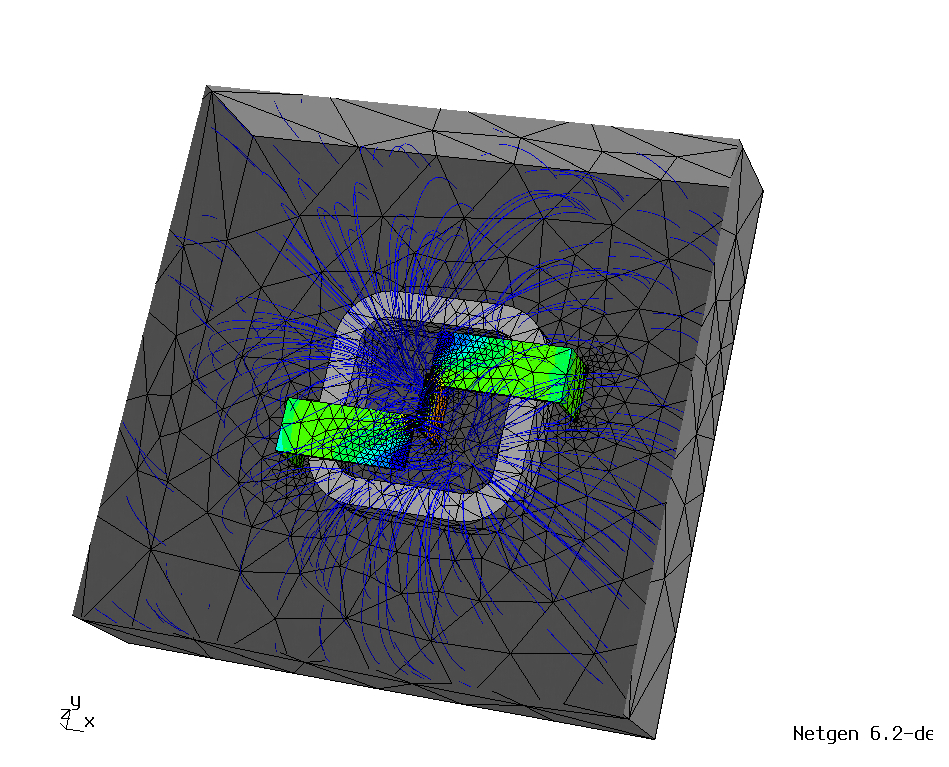
\includegraphics{halfmodel.jpg}
	\caption{Illustration of the the magnetic flux density in the steel
channels and magnetic field lines}
	\label{fig1}
\end{figure}
   
 

    \hypertarget{coding}{%
\section{Coding}\label{coding}}

\hypertarget{imports}{%
\subsection{Imports}\label{imports}}

Importing the packages \(\textit{ngsolve, netgen, numpy, ... }\) enables
all functionalities of this script. Additionally, the number of used
threads is reduced and the permeability of vacuum \(\mu_0\) is set.

    \begin{Verbatim}[commandchars=\\\{\}]
{\color{incolor}In [{\color{incolor}1}]:} \PY{k+kn}{from} \PY{n+nn}{ngsolve} \PY{k}{import} \PY{o}{*}
        \PY{k+kn}{from} \PY{n+nn}{netgen}\PY{n+nn}{.}\PY{n+nn}{csg} \PY{k}{import} \PY{o}{*}
        \PY{k+kn}{from} \PY{n+nn}{ngsolve}\PY{n+nn}{.}\PY{n+nn}{internal} \PY{k}{import} \PY{o}{*}
        
        \PY{k+kn}{import} \PY{n+nn}{numpy} \PY{k}{as} \PY{n+nn}{np}
        \PY{k+kn}{import} \PY{n+nn}{matplotlib}\PY{n+nn}{.}\PY{n+nn}{pyplot} \PY{k}{as} \PY{n+nn}{plt}
        \PY{k+kn}{import} \PY{n+nn}{matplotlib}
        \PY{k+kn}{import} \PY{n+nn}{time}
        
        \PY{n}{SetNumThreads}\PY{p}{(}\PY{l+m+mi}{10}\PY{p}{)}
        \PY{k+kn}{import} \PY{n+nn}{netgen}\PY{n+nn}{.}\PY{n+nn}{gui}
        
        \PY{n}{mu0} \PY{o}{=} \PY{l+m+mi}{4}\PY{o}{*}\PY{n}{np}\PY{o}{.}\PY{n}{pi}\PY{o}{*}\PY{l+m+mf}{1e\PYZhy{}7}
\end{Verbatim}

    \hypertarget{setting-arguments}{%
\subsection{Setting Arguments}\label{setting-arguments}}

First of all, the simulation parameters need to be set. The space order
defines the used order of the trial function and the test function
within the finite element space. The variable \(\texttt{I}_{ON}\)
defines the value of Ampere-turns in the coil. Considering the
Section \ref{problem-description}, the value for the Ampere-turns is set
to $ 1,000 $ or $ 3,000 $.

    \begin{Verbatim}[commandchars=\\\{\}]
{\color{incolor}In [{\color{incolor}2}]:} \PY{n}{space\PYZus{}order} \PY{o}{=} \PY{l+m+mi}{2}   
        \PY{n}{I0N} \PY{o}{=} \PY{l+m+mi}{1000}                  \PY{c+c1}{\PYZsh{} Ampere\PYZhy{}turns 1000 or 3000}
\end{Verbatim}

    \hypertarget{meshing}{%
\subsection{Meshing}\label{meshing}}

Next, the available mesh is loaded. The command \(Curve(5)\) determines
the roundness of the mesh and is obligatory for the provided geometry
with its curved corners.

    \begin{Verbatim}[commandchars=\\\{\}]
{\color{incolor}In [{\color{incolor}3}]:} \PY{n}{mesh} \PY{o}{=} \PY{n}{Mesh}\PY{p}{(}\PY{l+s+s2}{\PYZdq{}}\PY{l+s+s2}{./team13\PYZus{}mesh.vol}\PY{l+s+s2}{\PYZdq{}}\PY{p}{)}
        \PY{c+c1}{\PYZsh{} mesh = Mesh(\PYZdq{}./team13\PYZus{}mesh\PYZus{}full.vol\PYZdq{}) \PYZsh{} activate this to simulate the full problem}
        \PY{n}{mesh}\PY{o}{.}\PY{n}{Curve}\PY{p}{(}\PY{l+m+mi}{5}\PY{p}{)}
        
        \PY{c+c1}{\PYZsh{} check domains}
        \PY{n}{val} \PY{o}{=} \PY{p}{\PYZob{}}\PY{l+s+s2}{\PYZdq{}}\PY{l+s+s2}{corner\PYZus{}right\PYZus{}back}\PY{l+s+s2}{\PYZdq{}}\PY{p}{:}\PY{l+m+mi}{1} \PY{p}{,} \PY{l+s+s2}{\PYZdq{}}\PY{l+s+s2}{corner\PYZus{}left\PYZus{}back}\PY{l+s+s2}{\PYZdq{}}\PY{p}{:}\PY{l+m+mi}{1}\PY{p}{,} \PY{l+s+s2}{\PYZdq{}}\PY{l+s+s2}{corner\PYZus{}left\PYZus{}front}\PY{l+s+s2}{\PYZdq{}}\PY{p}{:}\PY{l+m+mi}{1}\PY{p}{,} \PY{l+s+s2}{\PYZdq{}}\PY{l+s+s2}{corner\PYZus{}right\PYZus{}front}\PY{l+s+s2}{\PYZdq{}}\PY{p}{:}\PY{l+m+mi}{1}\PY{p}{,} \PY{l+s+s2}{\PYZdq{}}\PY{l+s+s2}{brick\PYZus{}front}\PY{l+s+s2}{\PYZdq{}}\PY{p}{:}\PY{l+m+mi}{1}\PY{p}{,} \PY{l+s+s2}{\PYZdq{}}\PY{l+s+s2}{brick\PYZus{}back}\PY{l+s+s2}{\PYZdq{}}\PY{p}{:}\PY{l+m+mi}{1}\PY{p}{,} \PY{l+s+s2}{\PYZdq{}}\PY{l+s+s2}{brick\PYZus{}left}\PY{l+s+s2}{\PYZdq{}}\PY{p}{:}\PY{l+m+mi}{1}\PY{p}{,} \PY{l+s+s2}{\PYZdq{}}\PY{l+s+s2}{brick\PYZus{}right}\PY{l+s+s2}{\PYZdq{}}\PY{p}{:}\PY{l+m+mi}{1}\PY{p}{,} \PY{l+s+s2}{\PYZdq{}}\PY{l+s+s2}{iron}\PY{l+s+s2}{\PYZdq{}}\PY{p}{:}\PY{l+m+mi}{2}\PY{p}{,} \PY{l+s+s2}{\PYZdq{}}\PY{l+s+s2}{air}\PY{l+s+s2}{\PYZdq{}}\PY{p}{:}\PY{l+m+mf}{1.5}\PY{p}{\PYZcb{}}
        \PY{n}{domains} \PY{o}{=} \PY{n}{CoefficientFunction}\PY{p}{(}\PY{p}{[}\PY{n}{val}\PY{p}{[}\PY{n}{mat}\PY{p}{]} \PY{k}{if} \PY{n}{mat} \PY{o+ow}{in} \PY{n}{val}\PY{o}{.}\PY{n}{keys}\PY{p}{(}\PY{p}{)} \PY{k}{else} \PY{l+m+mi}{0} \PY{k}{for} \PY{n}{mat} \PY{o+ow}{in} \PY{n}{mesh}\PY{o}{.}\PY{n}{GetMaterials}\PY{p}{(}\PY{p}{)}\PY{p}{]}\PY{p}{)}
        \PY{n}{Draw}\PY{p}{(}\PY{n}{domains}\PY{p}{,} \PY{n}{mesh}\PY{p}{,} \PY{l+s+s2}{\PYZdq{}}\PY{l+s+s2}{domains}\PY{l+s+s2}{\PYZdq{}}\PY{p}{,} \PY{n}{draw\PYZus{}surf}\PY{o}{=}\PY{k+kc}{False}\PY{p}{)}
        
        \PY{c+c1}{\PYZsh{} some viewing optioins}
        \PY{n}{ngsolve}\PY{o}{.}\PY{n}{internal}\PY{o}{.}\PY{n}{viewoptions}\PY{o}{.}\PY{n}{clipping}\PY{o}{.}\PY{n}{notdomain}\PY{o}{=}\PY{l+m+mi}{1}
        \PY{n}{ngsolve}\PY{o}{.}\PY{n}{internal}\PY{o}{.}\PY{n}{visoptions}\PY{o}{.}\PY{n}{clipsolution}\PY{o}{=}\PY{l+s+s2}{\PYZdq{}}\PY{l+s+s2}{scal}\PY{l+s+s2}{\PYZdq{}}
        \PY{n}{ngsolve}\PY{o}{.}\PY{n}{internal}\PY{o}{.}\PY{n}{viewoptions}\PY{o}{.}\PY{n}{clipping}\PY{o}{.}\PY{n}{enable}\PY{o}{=}\PY{l+m+mi}{1}
        \PY{n}{ngsolve}\PY{o}{.}\PY{n}{internal}\PY{o}{.}\PY{n}{viewoptions}\PY{o}{.}\PY{n}{clipping}\PY{o}{.}\PY{n}{ny}\PY{o}{=}\PY{l+m+mi}{0}
        \PY{n}{ngsolve}\PY{o}{.}\PY{n}{internal}\PY{o}{.}\PY{n}{viewoptions}\PY{o}{.}\PY{n}{clipping}\PY{o}{.}\PY{n}{nz}\PY{o}{=}\PY{o}{\PYZhy{}}\PY{l+m+mi}{1}
        \PY{n}{ngsolve}\PY{o}{.}\PY{n}{internal}\PY{o}{.}\PY{n}{viewoptions}\PY{o}{.}\PY{n}{clipping}\PY{o}{.}\PY{n}{dist}\PY{o}{=}\PY{o}{\PYZhy{}}\PY{l+m+mf}{0.21}
        \PY{n}{ngsolve}\PY{o}{.}\PY{n}{internal}\PY{o}{.}\PY{n}{viewoptions}\PY{o}{.}\PY{n}{clipping}\PY{o}{.}\PY{n}{notdomain}\PY{o}{=}\PY{l+m+mi}{1}
        
        \PY{n}{Rotate}\PY{p}{(}\PY{l+m+mi}{0}\PY{p}{,} \PY{l+m+mi}{120}\PY{p}{)}
        
        \PY{n}{Redraw}\PY{p}{(}\PY{p}{)}
\end{Verbatim}

    To check the correct assignment of the domains \(\{air, iron, coil\}\),
all corresponding subdomains are coloured accordingly.
\begin{figure}[h]
	\centering
	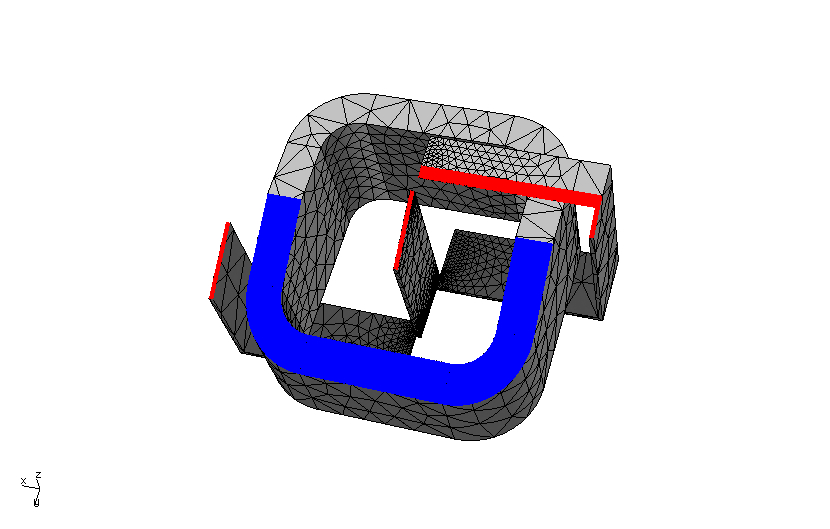
\includegraphics{geometry.jpg}
	\label{fig2}
	\caption{Illustration of the geometry}
\end{figure}
In Fig. 2 the coil is blue, the steel channels are red and the air is
transperent. For a meaningful display a clipping plane was inserted.

    \hypertarget{finite-element-space}{%
\subsection{Finite Element Space}\label{finite-element-space}}

The finite element space \(H(curl, \Omega)\) is selected and homogeneous
Dirichlet boundary conditions are prescribed on the far boundary.
Additionally * the solution, i.e.~magnetic vector potential
\(\textbf{A}\), is defined as \(\texttt{sol}\), * trial and test
function are introduced, * the \(\textit{CoefficientFunction}\)
\(\texttt{B}\) for the magnetic flux density is determined and *
\(\texttt{B}\) is drawn.

    \begin{Verbatim}[commandchars=\\\{\}]
{\color{incolor}In [{\color{incolor}4}]:} \PY{c+c1}{\PYZsh{} create fe space}
        \PY{n}{fes} \PY{o}{=} \PY{n}{HCurl}\PY{p}{(}\PY{n}{mesh}\PY{p}{,} \PY{n}{order}\PY{o}{=}\PY{n}{space\PYZus{}order}\PY{p}{,} \PY{n}{dirichlet}\PY{o}{=}\PY{l+s+s2}{\PYZdq{}}\PY{l+s+s2}{outer}\PY{l+s+s2}{\PYZdq{}}\PY{p}{,} \PY{n}{nograds}\PY{o}{=}\PY{k+kc}{True}\PY{p}{)}
        
        \PY{c+c1}{\PYZsh{} magnetic vector potential as GridFunction}
        \PY{n}{sol} \PY{o}{=} \PY{n}{GridFunction}\PY{p}{(}\PY{n}{fes}\PY{p}{,} \PY{l+s+s2}{\PYZdq{}}\PY{l+s+s2}{A}\PY{l+s+s2}{\PYZdq{}}\PY{p}{)}
        \PY{n}{sol}\PY{o}{.}\PY{n}{vec}\PY{p}{[}\PY{p}{:}\PY{p}{]} \PY{o}{=} \PY{l+m+mi}{0}
        
        \PY{c+c1}{\PYZsh{} Test\PYZhy{} and Trialfunction}
        \PY{n}{u} \PY{o}{=} \PY{n}{fes}\PY{o}{.}\PY{n}{TrialFunction}\PY{p}{(}\PY{p}{)}
        \PY{n}{v} \PY{o}{=} \PY{n}{fes}\PY{o}{.}\PY{n}{TestFunction}\PY{p}{(}\PY{p}{)}
        
        \PY{c+c1}{\PYZsh{} magnetic flux density}
        \PY{n}{B} \PY{o}{=} \PY{n}{curl}\PY{p}{(}\PY{n}{sol}\PY{p}{)}
        \PY{n}{Draw}\PY{p}{(}\PY{n}{B}\PY{p}{,} \PY{n}{mesh}\PY{p}{,} \PY{l+s+s2}{\PYZdq{}}\PY{l+s+s2}{B}\PY{l+s+s2}{\PYZdq{}}\PY{p}{,} \PY{n}{draw\PYZus{}surf}\PY{o}{=}\PY{k+kc}{False}\PY{p}{)}
\end{Verbatim}

    \hypertarget{material-parameters}{%
\subsection{Material Parameters}\label{material-parameters}}

The non-linear magnetisation curve of the material is defined in the
Section \ref{problem-description} .

    \begin{Verbatim}[commandchars=\\\{\}]
{\color{incolor}In [{\color{incolor}5}]:} \PY{n}{H\PYZus{}KL} \PY{o}{=} \PY{p}{[} \PY{o}{\PYZhy{}}\PY{l+m+mf}{4.47197834e\PYZhy{}13}\PY{p}{,} \PY{l+m+mf}{1.60000000e+01}\PY{p}{,} \PY{l+m+mf}{3.00000000e+01}\PY{p}{,} \PY{l+m+mf}{5.40000000e+01}\PYZbs{}
            \PY{p}{,} \PY{l+m+mf}{9.30000000e+01}\PY{p}{,} \PY{l+m+mf}{1.43000000e+02}\PY{p}{,} \PY{l+m+mf}{1.91000000e+02}\PY{p}{,} \PY{l+m+mf}{2.10000000e+02}\PYZbs{}
        \PY{p}{,} \PY{l+m+mf}{2.22000000e+02}\PY{p}{,} \PY{l+m+mf}{2.33000000e+02}\PY{p}{,} \PY{l+m+mf}{2.47000000e+02}\PY{p}{,} \PY{l+m+mf}{2.58000000e+02}\PYZbs{}
        \PY{p}{,} \PY{l+m+mf}{2.72000000e+02}\PY{p}{,} \PY{l+m+mf}{2.89000000e+02}\PY{p}{,} \PY{l+m+mf}{3.13000000e+02}\PY{p}{,} \PY{l+m+mf}{3.42000000e+02}\PYZbs{}
        \PY{p}{,} \PY{l+m+mf}{3.77000000e+02}\PY{p}{,} \PY{l+m+mf}{4.33000000e+02}\PY{p}{,} \PY{l+m+mf}{5.09000000e+02}\PY{p}{,} \PY{l+m+mf}{6.48000000e+02}\PYZbs{}
        \PY{p}{,} \PY{l+m+mf}{9.33000000e+02}\PY{p}{,} \PY{l+m+mf}{1.22800000e+03}\PY{p}{,} \PY{l+m+mf}{1.93400000e+03}\PY{p}{,} \PY{l+m+mf}{2.91300000e+03}\PYZbs{}
        \PY{p}{,} \PY{l+m+mf}{4.99300000e+03}\PY{p}{,} \PY{l+m+mf}{7.18900000e+03}\PY{p}{,} \PY{l+m+mf}{9.42300000e+03}\PY{p}{,} \PY{l+m+mf}{9.42300000e+03}\PYZbs{}
        \PY{p}{,} \PY{l+m+mf}{1.28203768e+04}\PY{p}{,} \PY{l+m+mf}{1.65447489e+04}\PY{p}{,} \PY{l+m+mf}{2.07163957e+04}\PY{p}{,} \PY{l+m+mf}{2.55500961e+04}\PYZbs{}
        \PY{p}{,} \PY{l+m+mf}{3.15206135e+04}\PY{p}{,} \PY{l+m+mf}{4.03204637e+04}\PY{p}{,} \PY{l+m+mf}{7.73038295e+04}\PY{p}{,} \PY{l+m+mf}{1.29272791e+05}\PYZbs{}
        \PY{p}{,} \PY{l+m+mf}{1.81241752e+05}\PY{p}{,} \PY{l+m+mf}{2.33210713e+05}\PY{p}{,} \PY{l+m+mf}{2.85179674e+05}\PY{p}{,} \PY{l+m+mf}{3.37148635e+05}\PYZbs{}
        \PY{p}{,} \PY{l+m+mf}{3.89117596e+05}\PY{p}{,} \PY{l+m+mf}{4.41086557e+05}\PY{p}{,} \PY{l+m+mf}{4.93055518e+05}\PY{p}{,} \PY{l+m+mf}{5.45024479e+05}\PYZbs{}
        \PY{p}{,} \PY{l+m+mf}{5.96993440e+05}\PY{p}{,} \PY{l+m+mf}{6.48962401e+05}\PY{p}{,} \PY{l+m+mf}{7.00931362e+05}\PY{p}{,} \PY{l+m+mf}{7.52900323e+05}\PYZbs{}
        \PY{p}{,} \PY{l+m+mf}{8.04869284e+05}\PY{p}{,} \PY{l+m+mf}{8.56838245e+05}\PY{p}{,} \PY{l+m+mf}{9.08807206e+05}\PY{p}{,} \PY{l+m+mf}{9.60776167e+05}\PYZbs{}
        \PY{p}{,} \PY{l+m+mf}{1.01274513e+06}\PY{p}{,} \PY{l+m+mf}{1.06471409e+06}\PY{p}{,} \PY{l+m+mf}{1.11668305e+06}\PY{p}{,} \PY{l+m+mf}{1.16865201e+06}\PYZbs{}
        \PY{p}{,} \PY{l+m+mf}{1.22062097e+06}\PY{p}{,} \PY{l+m+mf}{1.27258993e+06}\PY{p}{,} \PY{l+m+mf}{1.32455889e+06}\PY{p}{,} \PY{l+m+mf}{1.37652785e+06}\PYZbs{}
        \PY{p}{,} \PY{l+m+mf}{1.42849682e+06}\PY{p}{,} \PY{l+m+mf}{1.48046578e+06}\PY{p}{,} \PY{l+m+mf}{1.53243474e+06}\PY{p}{,} \PY{l+m+mf}{1.58440370e+06}\PYZbs{}
        \PY{p}{,} \PY{l+m+mf}{1.63637266e+06}\PY{p}{,} \PY{l+m+mf}{1.68834162e+06}\PY{p}{,} \PY{l+m+mf}{1.74031058e+06}\PY{p}{,} \PY{l+m+mf}{1.79227954e+06}\PYZbs{}
        \PY{p}{,} \PY{l+m+mf}{1.84424850e+06}\PY{p}{,} \PY{l+m+mf}{1.89621746e+06}\PY{p}{,} \PY{l+m+mf}{1.94818643e+06}\PY{p}{,} \PY{l+m+mf}{2.00015539e+06}\PYZbs{}
        \PY{p}{,} \PY{l+m+mf}{2.05212435e+06}\PY{p}{,} \PY{l+m+mf}{2.10409331e+06}\PY{p}{,} \PY{l+m+mf}{2.15606227e+06}\PY{p}{,} \PY{l+m+mf}{2.20803123e+06}\PYZbs{}
        \PY{p}{,} \PY{l+m+mf}{2.26000019e+06}\PY{p}{]}
        
        \PY{n}{B\PYZus{}KL} \PY{o}{=} \PY{p}{[}  \PY{l+m+mf}{0.00000000e+00}\PY{p}{,} \PY{l+m+mf}{2.50000000e\PYZhy{}03}\PY{p}{,} \PY{l+m+mf}{5.00000000e\PYZhy{}03}\PY{p}{,} \PY{l+m+mf}{1.25000000e\PYZhy{}02}\PYZbs{}
        \PY{p}{,} \PY{l+m+mf}{2.50000000e\PYZhy{}02}\PY{p}{,} \PY{l+m+mf}{5.00000000e\PYZhy{}02}\PY{p}{,} \PY{l+m+mf}{1.00000000e\PYZhy{}01}\PY{p}{,} \PY{l+m+mf}{2.00000000e\PYZhy{}01}\PYZbs{}
        \PY{p}{,} \PY{l+m+mf}{3.00000000e\PYZhy{}01}\PY{p}{,} \PY{l+m+mf}{4.00000000e\PYZhy{}01}\PY{p}{,} \PY{l+m+mf}{5.00000000e\PYZhy{}01}\PY{p}{,} \PY{l+m+mf}{6.00000000e\PYZhy{}01}\PYZbs{}
        \PY{p}{,} \PY{l+m+mf}{7.00000000e\PYZhy{}01}\PY{p}{,} \PY{l+m+mf}{8.00000000e\PYZhy{}01}\PY{p}{,} \PY{l+m+mf}{9.00000000e\PYZhy{}01}\PY{p}{,} \PY{l+m+mf}{1.00000000e+00}\PYZbs{}
        \PY{p}{,} \PY{l+m+mf}{1.10000000e+00}\PY{p}{,} \PY{l+m+mf}{1.20000000e+00}\PY{p}{,} \PY{l+m+mf}{1.30000000e+00}\PY{p}{,} \PY{l+m+mf}{1.40000000e+00}\PYZbs{}
        \PY{p}{,} \PY{l+m+mf}{1.50000000e+00}\PY{p}{,} \PY{l+m+mf}{1.55000000e+00}\PY{p}{,} \PY{l+m+mf}{1.60000000e+00}\PY{p}{,} \PY{l+m+mf}{1.65000000e+00}\PYZbs{}
        \PY{p}{,} \PY{l+m+mf}{1.70000000e+00}\PY{p}{,} \PY{l+m+mf}{1.75000000e+00}\PY{p}{,} \PY{l+m+mf}{1.80000000e+00}\PY{p}{,} \PY{l+m+mf}{1.80000000e+00}\PYZbs{}
        \PY{p}{,} \PY{l+m+mf}{1.86530612e+00}\PY{p}{,} \PY{l+m+mf}{1.93061224e+00}\PY{p}{,} \PY{l+m+mf}{1.99591837e+00}\PY{p}{,} \PY{l+m+mf}{2.06122449e+00}\PYZbs{}
        \PY{p}{,} \PY{l+m+mf}{2.12653061e+00}\PY{p}{,} \PY{l+m+mf}{2.19183673e+00}\PY{p}{,} \PY{l+m+mf}{2.25714286e+00}\PY{p}{,} \PY{l+m+mf}{2.32244898e+00}\PYZbs{}
        \PY{p}{,} \PY{l+m+mf}{2.38775510e+00}\PY{p}{,} \PY{l+m+mf}{2.45306122e+00}\PY{p}{,} \PY{l+m+mf}{2.51836735e+00}\PY{p}{,} \PY{l+m+mf}{2.58367347e+00}\PYZbs{}
        \PY{p}{,} \PY{l+m+mf}{2.64897959e+00}\PY{p}{,} \PY{l+m+mf}{2.71428571e+00}\PY{p}{,} \PY{l+m+mf}{2.77959184e+00}\PY{p}{,} \PY{l+m+mf}{2.84489796e+00}\PYZbs{}
        \PY{p}{,} \PY{l+m+mf}{2.91020408e+00}\PY{p}{,} \PY{l+m+mf}{2.97551020e+00}\PY{p}{,} \PY{l+m+mf}{3.04081633e+00}\PY{p}{,} \PY{l+m+mf}{3.10612245e+00}\PYZbs{}
        \PY{p}{,} \PY{l+m+mf}{3.17142857e+00}\PY{p}{,} \PY{l+m+mf}{3.23673469e+00}\PY{p}{,} \PY{l+m+mf}{3.30204082e+00}\PY{p}{,} \PY{l+m+mf}{3.36734694e+00}\PYZbs{}
        \PY{p}{,} \PY{l+m+mf}{3.43265306e+00}\PY{p}{,} \PY{l+m+mf}{3.49795918e+00}\PY{p}{,} \PY{l+m+mf}{3.56326531e+00}\PY{p}{,} \PY{l+m+mf}{3.62857143e+00}\PYZbs{}
        \PY{p}{,} \PY{l+m+mf}{3.69387755e+00}\PY{p}{,} \PY{l+m+mf}{3.75918367e+00}\PY{p}{,} \PY{l+m+mf}{3.82448980e+00}\PY{p}{,} \PY{l+m+mf}{3.88979592e+00}\PYZbs{}
        \PY{p}{,} \PY{l+m+mf}{3.95510204e+00}\PY{p}{,} \PY{l+m+mf}{4.02040816e+00}\PY{p}{,} \PY{l+m+mf}{4.08571429e+00}\PY{p}{,} \PY{l+m+mf}{4.15102041e+00}\PYZbs{}
        \PY{p}{,} \PY{l+m+mf}{4.21632653e+00}\PY{p}{,} \PY{l+m+mf}{4.28163265e+00}\PY{p}{,} \PY{l+m+mf}{4.34693878e+00}\PY{p}{,} \PY{l+m+mf}{4.41224490e+00}\PYZbs{}
        \PY{p}{,} \PY{l+m+mf}{4.47755102e+00}\PY{p}{,} \PY{l+m+mf}{4.54285714e+00}\PY{p}{,} \PY{l+m+mf}{4.60816327e+00}\PY{p}{,} \PY{l+m+mf}{4.67346939e+00}\PYZbs{}
        \PY{p}{,} \PY{l+m+mf}{4.73877551e+00}\PY{p}{,} \PY{l+m+mf}{4.80408163e+00}\PY{p}{,} \PY{l+m+mf}{4.86938776e+00}\PY{p}{,} \PY{l+m+mf}{4.93469388e+00}\PYZbs{}
        \PY{p}{,} \PY{l+m+mf}{5.00000000e+00}\PY{p}{]}
        \PY{n}{bh\PYZus{}curve} \PY{o}{=} \PY{n}{BSpline} \PY{p}{(}\PY{l+m+mi}{2}\PY{p}{,} \PY{p}{[}\PY{l+m+mi}{0}\PY{p}{]}\PY{o}{+}\PY{n+nb}{list}\PY{p}{(}\PY{n}{B\PYZus{}KL}\PY{p}{)}\PY{p}{,} \PY{n+nb}{list}\PY{p}{(}\PY{n}{H\PYZus{}KL}\PY{p}{)}\PY{p}{)} \PY{c+c1}{\PYZsh{} [0] + is needed!}
\end{Verbatim}

    \begin{Verbatim}[commandchars=\\\{\}]
{\color{incolor}In [{\color{incolor}6}]:} \PY{c+c1}{\PYZsh{} create figure}
        \PY{n}{plt}\PY{o}{.}\PY{n}{figure}\PY{p}{(}\PY{l+m+mi}{1}\PY{p}{,} \PY{n}{figsize}\PY{o}{=}\PY{p}{[}\PY{l+m+mi}{12}\PY{p}{,} \PY{l+m+mi}{9}\PY{p}{]}\PY{p}{)}
        \PY{n}{plt}\PY{o}{.}\PY{n}{clf}\PY{p}{(}\PY{p}{)}
        \PY{n}{plt}\PY{o}{.}\PY{n}{plot}\PY{p}{(}\PY{n}{H\PYZus{}KL}\PY{p}{,} \PY{n}{B\PYZus{}KL}\PY{p}{,} \PY{l+s+s1}{\PYZsq{}}\PY{l+s+s1}{.\PYZhy{}r}\PY{l+s+s1}{\PYZsq{}}\PY{p}{)}
        \PY{n}{plt}\PY{o}{.}\PY{n}{xlim}\PY{p}{(}\PY{l+m+mi}{0}\PY{p}{,} \PY{l+m+mi}{2000}\PY{p}{)}
        \PY{n}{plt}\PY{o}{.}\PY{n}{ylim}\PY{p}{(}\PY{l+m+mi}{0}\PY{p}{,} \PY{l+m+mf}{2.12}\PY{p}{)}
        \PY{n}{plt}\PY{o}{.}\PY{n}{grid}\PY{p}{(}\PY{p}{)}
        \PY{n}{plt}\PY{o}{.}\PY{n}{title}\PY{p}{(}\PY{l+s+s2}{\PYZdq{}}\PY{l+s+s2}{Magnetisation curve}\PY{l+s+s2}{\PYZdq{}}\PY{p}{)}
        \PY{n}{plt}\PY{o}{.}\PY{n}{xlabel}\PY{p}{(}\PY{l+s+s2}{\PYZdq{}}\PY{l+s+s2}{Magnetic Field Strength H  in  A/m}\PY{l+s+s2}{\PYZdq{}}\PY{p}{)}
        \PY{n}{plt}\PY{o}{.}\PY{n}{ylabel}\PY{p}{(}\PY{l+s+s2}{\PYZdq{}}\PY{l+s+s2}{Magnetic Flux Density B in T}\PY{l+s+s2}{\PYZdq{}}\PY{p}{)}
        \PY{n}{font} \PY{o}{=} \PY{p}{\PYZob{}}\PY{l+s+s1}{\PYZsq{}}\PY{l+s+s1}{size}\PY{l+s+s1}{\PYZsq{}}   \PY{p}{:} \PY{l+m+mi}{16}\PY{p}{\PYZcb{}}
        \PY{n}{matplotlib}\PY{o}{.}\PY{n}{rc}\PY{p}{(}\PY{l+s+s1}{\PYZsq{}}\PY{l+s+s1}{font}\PY{l+s+s1}{\PYZsq{}}\PY{p}{,} \PY{o}{*}\PY{o}{*}\PY{n}{font}\PY{p}{)}
        \PY{n}{plt}\PY{o}{.}\PY{n}{show}\PY{p}{(}\PY{n}{block}\PY{o}{=}\PY{k+kc}{False}\PY{p}{)}
\end{Verbatim}

    \begin{center}
    \adjustimage{max size={0.9\linewidth}{0.9\paperheight}}{output_15_0.png}
    \end{center}
    { \hspace*{\fill} \\}
    
    The non-linear problem is solved by minimising the the functional


\begin{equation}
 F(\textbf{A}) = \int_{\Omega}w(|\nabla\times \textbf{A}|)\;d\Omega - \int_{\Omega_c}\textbf{J}\cdot \textbf{A}\;d\Omega.
\end{equation}


Therefore the magnetic energy density


\begin{equation}
    w(B) = \int_0^B H(B')\;dB' 
\end{equation}


has to be set

    \begin{Verbatim}[commandchars=\\\{\}]
{\color{incolor}In [{\color{incolor}7}]:} \PY{n}{energy\PYZus{}dens} \PY{o}{=} \PY{n}{bh\PYZus{}curve}\PY{o}{.}\PY{n}{Integrate}\PY{p}{(}\PY{p}{)}    \PY{c+c1}{\PYZsh{} to be minimised}
\end{Verbatim}

    \hypertarget{stiffness-matrix-and-dirichlet-boundaries}{%
\subsection{Stiffness Matrix and Dirichlet
Boundaries}\label{stiffness-matrix-and-dirichlet-boundaries}}

The stiffness matrix is set on all regions and the regularisation term
mentioned in the section Section \ref{problem-description} is added.

    \begin{Verbatim}[commandchars=\\\{\}]
{\color{incolor}In [{\color{incolor}8}]:} \PY{n}{a} \PY{o}{=} \PY{n}{BilinearForm}\PY{p}{(}\PY{n}{fes}\PY{p}{,} \PY{n}{symmetric}\PY{o}{=}\PY{k+kc}{True}\PY{p}{)}
        
        \PY{n}{a} \PY{o}{+}\PY{o}{=} \PY{n}{SymbolicBFI}\PY{p}{(}\PY{l+m+mi}{1}\PY{o}{/}\PY{n}{mu0} \PY{o}{*} \PY{n}{curl}\PY{p}{(}\PY{n}{u}\PY{p}{)}\PY{o}{*}\PY{n}{curl}\PY{p}{(}\PY{n}{v}\PY{p}{)}\PY{p}{,} \PY{n}{definedon}\PY{o}{=}\PY{o}{\PYZti{}}\PY{n}{mesh}\PY{o}{.}\PY{n}{Materials}\PY{p}{(}\PY{l+s+s2}{\PYZdq{}}\PY{l+s+s2}{iron}\PY{l+s+s2}{\PYZdq{}}\PY{p}{)}\PY{p}{)}
        \PY{n}{a} \PY{o}{+}\PY{o}{=} \PY{n}{SymbolicEnergy}\PY{p}{(}\PY{n}{energy\PYZus{}dens}\PY{p}{(}\PY{n}{sqrt}\PY{p}{(}\PY{l+m+mf}{1e\PYZhy{}12}\PY{o}{+}\PY{n}{curl}\PY{p}{(}\PY{n}{u}\PY{p}{)}\PY{o}{*}\PY{n}{curl}\PY{p}{(}\PY{n}{u}\PY{p}{)}\PY{p}{)}\PY{p}{)}\PY{p}{,} \PY{n}{definedon}\PY{o}{=}\PY{n}{mesh}\PY{o}{.}\PY{n}{Materials}\PY{p}{(}\PY{l+s+s2}{\PYZdq{}}\PY{l+s+s2}{iron}\PY{l+s+s2}{\PYZdq{}}\PY{p}{)}\PY{p}{)} \PY{c+c1}{\PYZsh{} 1e\PYZhy{}12 ... to avoid 0}
        \PY{n}{a} \PY{o}{+}\PY{o}{=} \PY{n}{SymbolicBFI}\PY{p}{(}\PY{l+m+mf}{1e\PYZhy{}1}\PY{o}{*}\PY{n}{u}\PY{o}{*}\PY{n}{v}\PY{p}{)}  \PY{c+c1}{\PYZsh{} regularisation}
        
        \PY{c+c1}{\PYZsh{} preconditioner}
        \PY{n}{c} \PY{o}{=} \PY{n}{Preconditioner}\PY{p}{(}\PY{n}{a}\PY{p}{,} \PY{n+nb}{type}\PY{o}{=}\PY{l+s+s2}{\PYZdq{}}\PY{l+s+s2}{direct}\PY{l+s+s2}{\PYZdq{}}\PY{p}{,} \PY{n}{inverse}\PY{o}{=}\PY{l+s+s2}{\PYZdq{}}\PY{l+s+s2}{sparsecholesky}\PY{l+s+s2}{\PYZdq{}}\PY{p}{)}
\end{Verbatim}

    The boundary condition


\begin{equation}
    \textbf{B}\cdot\textbf{n} = 0
\end{equation}

is prescribed with the magnetic vector potential by

\begin{align}
    \nabla\times\textbf{A} \cdot\textbf{n} &= 0\\
    \textbf{A} &= \textbf{0}\qquad\text{on }\Gamma_{outer}.
\end{align}


    \hypertarget{biot-savart-field-and-neumann-boundaries}{%
\subsection{Biot-Savart Field and Neumann
Boundaries}\label{biot-savart-field-and-neumann-boundaries}}

In this section, the impressed current density in the coil is modelled.
This has to be done carefully, since the orientation of the current has
to be defined in the curved corners consistently.

Without details:

    \begin{Verbatim}[commandchars=\\\{\}]
{\color{incolor}In [{\color{incolor}9}]:} \PY{n}{A} \PY{o}{=} \PY{l+m+mi}{2500}\PY{o}{*}\PY{l+m+mf}{1e\PYZhy{}6}       
        \PY{n}{J0} \PY{o}{=} \PY{n}{I0N}\PY{o}{/}\PY{n}{A}
        \PY{c+c1}{\PYZsh{} +++ bricks +++}
        \PY{n}{J\PYZus{}brick\PYZus{}back} \PY{o}{=} \PY{p}{[}\PY{l+m+mi}{1}\PY{p}{,} \PY{l+m+mi}{0}\PY{p}{]}
        \PY{n}{J\PYZus{}brick\PYZus{}front} \PY{o}{=} \PY{p}{[}\PY{o}{\PYZhy{}}\PY{l+m+mi}{1}\PY{p}{,} \PY{l+m+mi}{0}\PY{p}{]}
        \PY{n}{J\PYZus{}brick\PYZus{}left} \PY{o}{=} \PY{p}{[}\PY{l+m+mi}{0}\PY{p}{,} \PY{l+m+mi}{1}\PY{p}{]}
        \PY{n}{J\PYZus{}brick\PYZus{}right} \PY{o}{=} \PY{p}{[}\PY{l+m+mi}{0}\PY{p}{,} \PY{o}{\PYZhy{}}\PY{l+m+mi}{1}\PY{p}{]}
        
        \PY{c+c1}{\PYZsh{} +++ corners +++}
        \PY{c+c1}{\PYZsh{} right back}
        \PY{n}{x\PYZus{}right\PYZus{}back} \PY{o}{=} \PY{n}{x} \PY{o}{\PYZhy{}} \PY{l+m+mf}{0.050}
        \PY{n}{y\PYZus{}right\PYZus{}back} \PY{o}{=} \PY{n}{y} \PY{o}{\PYZhy{}} \PY{l+m+mf}{0.050}
        \PY{n}{r\PYZus{}right\PYZus{}back} \PY{o}{=} \PY{p}{(}\PY{n}{x\PYZus{}right\PYZus{}back}\PY{o}{*}\PY{o}{*}\PY{l+m+mi}{2} \PY{o}{+} \PY{n}{y\PYZus{}right\PYZus{}back}\PY{o}{*}\PY{o}{*}\PY{l+m+mi}{2}\PY{p}{)}\PY{o}{*}\PY{o}{*}\PY{p}{(}\PY{l+m+mi}{1}\PY{o}{/}\PY{l+m+mi}{2}\PY{p}{)}
        \PY{n}{J\PYZus{}corner\PYZus{}right\PYZus{}back} \PY{o}{=} \PY{p}{[}\PY{l+m+mi}{1}\PY{o}{/}\PY{n}{r\PYZus{}right\PYZus{}back} \PY{o}{*} \PY{n}{y\PYZus{}right\PYZus{}back}\PY{p}{,} \PY{o}{\PYZhy{}}\PY{l+m+mi}{1}\PY{o}{/}\PY{n}{r\PYZus{}right\PYZus{}back} \PY{o}{*} \PY{n}{x\PYZus{}right\PYZus{}back}\PY{p}{]}
        
        \PY{c+c1}{\PYZsh{} left back}
        \PY{n}{x\PYZus{}left\PYZus{}back} \PY{o}{=} \PY{n}{x} \PY{o}{+} \PY{l+m+mf}{0.050}
        \PY{n}{y\PYZus{}left\PYZus{}back} \PY{o}{=} \PY{n}{y} \PY{o}{\PYZhy{}} \PY{l+m+mf}{0.050}
        \PY{n}{r\PYZus{}left\PYZus{}back} \PY{o}{=} \PY{p}{(}\PY{n}{x\PYZus{}left\PYZus{}back}\PY{o}{*}\PY{o}{*}\PY{l+m+mi}{2} \PY{o}{+} \PY{n}{y\PYZus{}left\PYZus{}back}\PY{o}{*}\PY{o}{*}\PY{l+m+mi}{2}\PY{p}{)}\PY{o}{*}\PY{o}{*}\PY{p}{(}\PY{l+m+mi}{1}\PY{o}{/}\PY{l+m+mi}{2}\PY{p}{)}
        \PY{n}{J\PYZus{}corner\PYZus{}left\PYZus{}back} \PY{o}{=}  \PY{p}{[}\PY{l+m+mi}{1}\PY{o}{/}\PY{n}{r\PYZus{}left\PYZus{}back} \PY{o}{*} \PY{n}{y\PYZus{}left\PYZus{}back}\PY{p}{,} \PY{o}{\PYZhy{}}\PY{l+m+mi}{1}\PY{o}{/}\PY{n}{r\PYZus{}left\PYZus{}back} \PY{o}{*} \PY{n}{x\PYZus{}left\PYZus{}back}\PY{p}{]}
        
        
        \PY{c+c1}{\PYZsh{} left front}
        \PY{n}{x\PYZus{}left\PYZus{}front} \PY{o}{=} \PY{n}{x} \PY{o}{+} \PY{l+m+mf}{0.050}
        \PY{n}{y\PYZus{}left\PYZus{}front} \PY{o}{=} \PY{n}{y} \PY{o}{+} \PY{l+m+mf}{0.050}
        \PY{n}{r\PYZus{}left\PYZus{}front} \PY{o}{=} \PY{p}{(}\PY{n}{x\PYZus{}left\PYZus{}front}\PY{o}{*}\PY{o}{*}\PY{l+m+mi}{2} \PY{o}{+} \PY{n}{y\PYZus{}left\PYZus{}front}\PY{o}{*}\PY{o}{*}\PY{l+m+mi}{2}\PY{p}{)}\PY{o}{*}\PY{o}{*}\PY{p}{(}\PY{l+m+mi}{1}\PY{o}{/}\PY{l+m+mi}{2}\PY{p}{)}
        \PY{n}{J\PYZus{}corner\PYZus{}left\PYZus{}front} \PY{o}{=} \PY{p}{[}\PY{l+m+mi}{1}\PY{o}{/}\PY{n}{r\PYZus{}left\PYZus{}front} \PY{o}{*} \PY{n}{y\PYZus{}left\PYZus{}front}\PY{p}{,} \PY{o}{\PYZhy{}}\PY{l+m+mi}{1}\PY{o}{/}\PY{n}{r\PYZus{}left\PYZus{}front} \PY{o}{*} \PY{n}{x\PYZus{}left\PYZus{}front}\PY{p}{]}
        
        \PY{c+c1}{\PYZsh{} right front}
        \PY{n}{x\PYZus{}right\PYZus{}front} \PY{o}{=} \PY{n}{x} \PY{o}{\PYZhy{}} \PY{l+m+mf}{0.050}
        \PY{n}{y\PYZus{}right\PYZus{}front} \PY{o}{=} \PY{n}{y} \PY{o}{+} \PY{l+m+mf}{0.050}
        \PY{n}{r\PYZus{}right\PYZus{}front} \PY{o}{=} \PY{p}{(}\PY{n}{x\PYZus{}right\PYZus{}front}\PY{o}{*}\PY{o}{*}\PY{l+m+mi}{2} \PY{o}{+} \PY{n}{y\PYZus{}right\PYZus{}front}\PY{o}{*}\PY{o}{*}\PY{l+m+mi}{2}\PY{p}{)}\PY{o}{*}\PY{o}{*}\PY{p}{(}\PY{l+m+mi}{1}\PY{o}{/}\PY{l+m+mi}{2}\PY{p}{)}
        \PY{n}{J\PYZus{}corner\PYZus{}right\PYZus{}front} \PY{o}{=} \PY{p}{[}\PY{l+m+mi}{1}\PY{o}{/}\PY{n}{r\PYZus{}right\PYZus{}front} \PY{o}{*} \PY{n}{y\PYZus{}right\PYZus{}front}\PY{p}{,} \PY{o}{\PYZhy{}}\PY{l+m+mi}{1}\PY{o}{/}\PY{n}{r\PYZus{}right\PYZus{}front} \PY{o}{*} \PY{n}{x\PYZus{}right\PYZus{}front}\PY{p}{]}
        
        \PY{c+c1}{\PYZsh{} J}
        \PY{n}{val}\PY{o}{=}\PY{p}{\PYZob{}}   \PY{l+s+s2}{\PYZdq{}}\PY{l+s+s2}{corner\PYZus{}right\PYZus{}back}\PY{l+s+s2}{\PYZdq{}}\PY{p}{:}\PY{n}{J\PYZus{}corner\PYZus{}right\PYZus{}back}\PY{p}{,} \PY{l+s+s2}{\PYZdq{}}\PY{l+s+s2}{corner\PYZus{}left\PYZus{}back}\PY{l+s+s2}{\PYZdq{}}\PY{p}{:}\PY{n}{J\PYZus{}corner\PYZus{}left\PYZus{}back}\PY{p}{,} \PYZbs{}
                \PY{l+s+s2}{\PYZdq{}}\PY{l+s+s2}{corner\PYZus{}left\PYZus{}front}\PY{l+s+s2}{\PYZdq{}}\PY{p}{:}\PY{n}{J\PYZus{}corner\PYZus{}left\PYZus{}front}\PY{p}{,} \PY{l+s+s2}{\PYZdq{}}\PY{l+s+s2}{corner\PYZus{}right\PYZus{}front}\PY{l+s+s2}{\PYZdq{}}\PY{p}{:}\PY{n}{J\PYZus{}corner\PYZus{}right\PYZus{}front}\PY{p}{,}\PYZbs{}
                \PY{l+s+s2}{\PYZdq{}}\PY{l+s+s2}{brick\PYZus{}back}\PY{l+s+s2}{\PYZdq{}}\PY{p}{:}\PY{n}{J\PYZus{}brick\PYZus{}back}\PY{p}{,} \PY{l+s+s2}{\PYZdq{}}\PY{l+s+s2}{brick\PYZus{}left}\PY{l+s+s2}{\PYZdq{}}\PY{p}{:}\PY{n}{J\PYZus{}brick\PYZus{}left}\PY{p}{,} \PYZbs{}
                \PY{l+s+s2}{\PYZdq{}}\PY{l+s+s2}{brick\PYZus{}front}\PY{l+s+s2}{\PYZdq{}}\PY{p}{:}\PY{n}{J\PYZus{}brick\PYZus{}front}\PY{p}{,} \PY{l+s+s2}{\PYZdq{}}\PY{l+s+s2}{brick\PYZus{}right}\PY{l+s+s2}{\PYZdq{}}\PY{p}{:}\PY{n}{J\PYZus{}brick\PYZus{}right}\PY{p}{\PYZcb{}}    
        
        \PY{n}{J} \PY{o}{=} \PY{n}{J0} \PY{o}{*} \PY{n}{CoefficientFunction}\PY{p}{(}\PY{p}{[}\PY{n}{val}\PY{p}{[}\PY{n}{mat}\PY{p}{]}\PY{p}{[}\PY{l+m+mi}{0}\PY{p}{]} \PY{k}{if} \PY{n}{mat} \PY{o+ow}{in} \PY{n}{val}\PY{o}{.}\PY{n}{keys}\PY{p}{(}\PY{p}{)} \PY{k}{else} \PY{l+m+mi}{0} \PY{k}{for} \PY{n}{mat} \PY{o+ow}{in} \PY{n}{mesh}\PY{o}{.}\PY{n}{GetMaterials}\PY{p}{(}\PY{p}{)}\PY{p}{]}\PY{p}{)}\PY{o}{*}\PY{n}{CoefficientFunction}\PY{p}{(}\PY{p}{(}\PY{l+m+mi}{1}\PY{p}{,}\PY{l+m+mi}{0}\PY{p}{,}\PY{l+m+mi}{0}\PY{p}{)}\PY{p}{)} \PY{o}{+} \PYZbs{}
            \PY{n}{J0} \PY{o}{*} \PY{n}{CoefficientFunction}\PY{p}{(}\PY{p}{[}\PY{n}{val}\PY{p}{[}\PY{n}{mat}\PY{p}{]}\PY{p}{[}\PY{l+m+mi}{1}\PY{p}{]} \PY{k}{if} \PY{n}{mat} \PY{o+ow}{in} \PY{n}{val}\PY{o}{.}\PY{n}{keys}\PY{p}{(}\PY{p}{)} \PY{k}{else} \PY{l+m+mi}{0} \PY{k}{for} \PY{n}{mat} \PY{o+ow}{in} \PY{n}{mesh}\PY{o}{.}\PY{n}{GetMaterials}\PY{p}{(}\PY{p}{)}\PY{p}{]}\PY{p}{)}\PY{o}{*}\PY{n}{CoefficientFunction}\PY{p}{(}\PY{p}{(}\PY{l+m+mi}{0}\PY{p}{,}\PY{l+m+mi}{1}\PY{p}{,}\PY{l+m+mi}{0}\PY{p}{)}\PY{p}{)}
        
        \PY{n}{Draw}\PY{p}{(}\PY{n}{J}\PY{p}{,} \PY{n}{mesh}\PY{p}{,} \PY{l+s+s2}{\PYZdq{}}\PY{l+s+s2}{J}\PY{l+s+s2}{\PYZdq{}}\PY{p}{)}
\end{Verbatim}

    \begin{Verbatim}[commandchars=\\\{\}]
{\color{incolor}In [{\color{incolor}10}]:} \PY{c+c1}{\PYZsh{} figure}
         \PY{n}{Nx} \PY{o}{=} \PY{l+m+mi}{30}
         \PY{n}{Ny} \PY{o}{=} \PY{l+m+mi}{30}
         \PY{n}{xi} \PY{o}{=} \PY{n}{np}\PY{o}{.}\PY{n}{linspace}\PY{p}{(}\PY{o}{\PYZhy{}}\PY{l+m+mf}{0.100}\PY{p}{,} \PY{l+m+mf}{0.100}\PY{p}{,} \PY{n}{Nx}\PY{p}{)}
         \PY{n}{yi} \PY{o}{=} \PY{n}{np}\PY{o}{.}\PY{n}{linspace}\PY{p}{(}\PY{o}{\PYZhy{}}\PY{l+m+mf}{0.100}\PY{p}{,} \PY{l+m+mf}{0.100}\PY{p}{,} \PY{n}{Ny}\PY{p}{)}
         
         \PY{n}{X}\PY{p}{,} \PY{n}{Y}\PY{o}{=} \PY{n}{np}\PY{o}{.}\PY{n}{meshgrid}\PY{p}{(}\PY{n}{xi}\PY{p}{,} \PY{n}{yi}\PY{p}{)}
         \PY{n}{J\PYZus{}T} \PY{o}{=} \PY{n}{np}\PY{o}{.}\PY{n}{zeros}\PY{p}{(}\PY{p}{[}\PY{n}{Nx}\PY{p}{,} \PY{n}{Ny}\PY{p}{,} \PY{l+m+mi}{2}\PY{p}{]}\PY{p}{)}
         
         \PY{k}{for} \PY{n}{i} \PY{o+ow}{in} \PY{n+nb}{range}\PY{p}{(}\PY{n}{Nx}\PY{p}{)}\PY{p}{:}
             \PY{k}{for} \PY{n}{j} \PY{o+ow}{in} \PY{n+nb}{range}\PY{p}{(}\PY{n}{Ny}\PY{p}{)}\PY{p}{:}
                 \PY{n}{tmp} \PY{o}{=} \PY{n}{J}\PY{p}{(}\PY{n}{mesh}\PY{p}{(}\PY{n}{xi}\PY{p}{[}\PY{n}{i}\PY{p}{]}\PY{p}{,} \PY{n}{yi}\PY{p}{[}\PY{n}{j}\PY{p}{]}\PY{p}{,} \PY{l+m+mi}{0}\PY{p}{)}\PY{p}{)}
                 \PY{n}{J\PYZus{}T}\PY{p}{[}\PY{n}{i}\PY{p}{,} \PY{n}{j}\PY{p}{,} \PY{l+m+mi}{0}\PY{p}{]} \PY{o}{=} \PY{n}{tmp}\PY{p}{[}\PY{l+m+mi}{0}\PY{p}{]}
                 \PY{n}{J\PYZus{}T}\PY{p}{[}\PY{n}{i}\PY{p}{,} \PY{n}{j}\PY{p}{,} \PY{l+m+mi}{1}\PY{p}{]} \PY{o}{=} \PY{n}{tmp}\PY{p}{[}\PY{l+m+mi}{1}\PY{p}{]}
         \PY{n}{J\PYZus{}T}\PY{p}{[}\PY{p}{:}\PY{p}{,} \PY{p}{:}\PY{p}{,} \PY{l+m+mi}{0}\PY{p}{]} \PY{o}{=} \PY{n}{np}\PY{o}{.}\PY{n}{transpose}\PY{p}{(}\PY{n}{J\PYZus{}T}\PY{p}{[}\PY{p}{:}\PY{p}{,} \PY{p}{:}\PY{p}{,} \PY{l+m+mi}{0}\PY{p}{]}\PY{p}{)}
         \PY{n}{J\PYZus{}T}\PY{p}{[}\PY{p}{:}\PY{p}{,} \PY{p}{:}\PY{p}{,} \PY{l+m+mi}{1}\PY{p}{]} \PY{o}{=} \PY{n}{np}\PY{o}{.}\PY{n}{transpose}\PY{p}{(}\PY{n}{J\PYZus{}T}\PY{p}{[}\PY{p}{:}\PY{p}{,} \PY{p}{:}\PY{p}{,} \PY{l+m+mi}{1}\PY{p}{]}\PY{p}{)}
         \PY{n}{plt}\PY{o}{.}\PY{n}{figure}\PY{p}{(}\PY{l+m+mi}{1}\PY{p}{,} \PY{n}{figsize}\PY{o}{=}\PY{p}{[}\PY{l+m+mi}{10}\PY{p}{,} \PY{l+m+mi}{10}\PY{p}{]}\PY{p}{)}
         \PY{n}{plt}\PY{o}{.}\PY{n}{quiver}\PY{p}{(}\PY{n}{X}\PY{p}{,} \PY{n}{Y}\PY{p}{,} \PY{n}{J\PYZus{}T}\PY{p}{[}\PY{p}{:}\PY{p}{,} \PY{p}{:}\PY{p}{,} \PY{l+m+mi}{0}\PY{p}{]}\PY{p}{,} \PY{n}{J\PYZus{}T}\PY{p}{[}\PY{p}{:}\PY{p}{,} \PY{p}{:}\PY{p}{,} \PY{l+m+mi}{1}\PY{p}{]}\PY{p}{)}
         \PY{n}{plt}\PY{o}{.}\PY{n}{xlabel}\PY{p}{(}\PY{l+s+s2}{\PYZdq{}}\PY{l+s+s2}{x coordinate / m}\PY{l+s+s2}{\PYZdq{}}\PY{p}{)}
         \PY{n}{plt}\PY{o}{.}\PY{n}{ylabel}\PY{p}{(}\PY{l+s+s2}{\PYZdq{}}\PY{l+s+s2}{y coordinate / m}\PY{l+s+s2}{\PYZdq{}}\PY{p}{)}
         \PY{n}{plt}\PY{o}{.}\PY{n}{title}\PY{p}{(}\PY{l+s+s2}{\PYZdq{}}\PY{l+s+s2}{Biot\PYZhy{}Savart Field}\PY{l+s+s2}{\PYZdq{}}\PY{p}{)}
         \PY{n}{plt}\PY{o}{.}\PY{n}{xlim}\PY{p}{(}\PY{p}{[}\PY{o}{\PYZhy{}}\PY{l+m+mf}{0.1}\PY{p}{,} \PY{l+m+mf}{0.1}\PY{p}{]}\PY{p}{)}
         \PY{n}{plt}\PY{o}{.}\PY{n}{ylim}\PY{p}{(}\PY{p}{[}\PY{o}{\PYZhy{}}\PY{l+m+mf}{0.1}\PY{p}{,} \PY{l+m+mf}{0.1}\PY{p}{]}\PY{p}{)}
         \PY{n}{font} \PY{o}{=} \PY{p}{\PYZob{}}\PY{l+s+s1}{\PYZsq{}}\PY{l+s+s1}{size}\PY{l+s+s1}{\PYZsq{}}   \PY{p}{:} \PY{l+m+mi}{16}\PY{p}{\PYZcb{}}
         \PY{n}{matplotlib}\PY{o}{.}\PY{n}{rc}\PY{p}{(}\PY{l+s+s1}{\PYZsq{}}\PY{l+s+s1}{font}\PY{l+s+s1}{\PYZsq{}}\PY{p}{,} \PY{o}{*}\PY{o}{*}\PY{n}{font}\PY{p}{)}
         \PY{n}{plt}\PY{o}{.}\PY{n}{show}\PY{p}{(}\PY{n}{block}\PY{o}{=}\PY{k+kc}{False}\PY{p}{)}
\end{Verbatim}

    \begin{center}
    \adjustimage{max size={0.9\linewidth}{0.9\paperheight}}{output_23_0.png}
    \end{center}
    { \hspace*{\fill} \\}
    
    The absolute value of the current density \(|\textbf{J}|\) is constant
in the whole volume of the coil. The \(\textit{CoefficientFunction}\)
\(\texttt{J}\) is used for the right-hand side of the weak formulation.

    \begin{Verbatim}[commandchars=\\\{\}]
{\color{incolor}In [{\color{incolor}11}]:} \PY{n}{f} \PY{o}{=} \PY{n}{LinearForm}\PY{p}{(}\PY{n}{fes}\PY{p}{)}
         \PY{n}{f} \PY{o}{+}\PY{o}{=} \PY{n}{SymbolicLFI}\PY{p}{(}\PY{n}{J}\PY{o}{*}\PY{n}{v}\PY{p}{)}
\end{Verbatim}

    \hypertarget{solving-the-problem}{%
\subsection{Solving the Problem}\label{solving-the-problem}}

The problem is iteratively solved by finding the
\href{https://ngsolve.org/docu/latest/i-tutorials/unit-3.8-nonlmin/nonlmin.html}{minimum
energy} until an error falls bellow a specified limit.

    \begin{Verbatim}[commandchars=\\\{\}]
{\color{incolor}In [{\color{incolor}12}]:} \PY{n}{t\PYZus{}simulation} \PY{o}{=} \PY{n}{time}\PY{o}{.}\PY{n}{time}\PY{p}{(}\PY{p}{)}
         \PY{k}{with} \PY{n}{TaskManager}\PY{p}{(}\PY{p}{)}\PY{p}{:}
             \PY{n}{f}\PY{o}{.}\PY{n}{Assemble}\PY{p}{(}\PY{p}{)}
             
             \PY{n}{err} \PY{o}{=} \PY{l+m+mi}{1}
             \PY{n}{it} \PY{o}{=} \PY{l+m+mi}{1}
             
             \PY{c+c1}{\PYZsh{} create memories}
             \PY{n}{au} \PY{o}{=} \PY{n}{sol}\PY{o}{.}\PY{n}{vec}\PY{o}{.}\PY{n}{CreateVector}\PY{p}{(}\PY{p}{)}
             \PY{n}{r} \PY{o}{=} \PY{n}{sol}\PY{o}{.}\PY{n}{vec}\PY{o}{.}\PY{n}{CreateVector}\PY{p}{(}\PY{p}{)}
             \PY{n}{w} \PY{o}{=} \PY{n}{sol}\PY{o}{.}\PY{n}{vec}\PY{o}{.}\PY{n}{CreateVector}\PY{p}{(}\PY{p}{)}
             \PY{n}{sol\PYZus{}new} \PY{o}{=} \PY{n}{sol}\PY{o}{.}\PY{n}{vec}\PY{o}{.}\PY{n}{CreateVector}\PY{p}{(}\PY{p}{)}
         
             \PY{k}{while} \PY{n}{err} \PY{o}{\PYZgt{}} \PY{l+m+mf}{1e\PYZhy{}10}\PY{p}{:}
                 \PY{n+nb}{print} \PY{p}{(}\PY{l+s+s2}{\PYZdq{}}\PY{l+s+s2}{nonlinear iteration}\PY{l+s+s2}{\PYZdq{}}\PY{p}{,} \PY{n}{it}\PY{p}{)}
                 \PY{n}{it} \PY{o}{=} \PY{n}{it}\PY{o}{+}\PY{l+m+mi}{1}
         
                 \PY{c+c1}{\PYZsh{} calculate current energy}
                 \PY{n}{E0} \PY{o}{=} \PY{n}{a}\PY{o}{.}\PY{n}{Energy}\PY{p}{(}\PY{n}{sol}\PY{o}{.}\PY{n}{vec}\PY{p}{)} \PY{o}{\PYZhy{}} \PY{n}{InnerProduct}\PY{p}{(}\PY{n}{f}\PY{o}{.}\PY{n}{vec}\PY{p}{,} \PY{n}{sol}\PY{o}{.}\PY{n}{vec}\PY{p}{)}
                 \PY{n+nb}{print} \PY{p}{(}\PY{l+s+s2}{\PYZdq{}}\PY{l+s+s2}{Energy old = }\PY{l+s+s2}{\PYZdq{}}\PY{p}{,} \PY{n}{E0}\PY{p}{)}
                 
                 \PY{c+c1}{\PYZsh{} solve linearized problem}
                 \PY{n}{a}\PY{o}{.}\PY{n}{AssembleLinearization}\PY{p}{(}\PY{n}{sol}\PY{o}{.}\PY{n}{vec}\PY{p}{)}
             
                 \PY{n}{a}\PY{o}{.}\PY{n}{Apply} \PY{p}{(}\PY{n}{sol}\PY{o}{.}\PY{n}{vec}\PY{p}{,} \PY{n}{au}\PY{p}{)}
                 \PY{n}{r}\PY{o}{.}\PY{n}{data} \PY{o}{=} \PY{n}{f}\PY{o}{.}\PY{n}{vec} \PY{o}{\PYZhy{}} \PY{n}{au}
         
                 \PY{c+c1}{\PYZsh{} inverse of a}
                 \PY{n}{inv} \PY{o}{=} \PY{n}{CGSolver} \PY{p}{(}\PY{n}{mat}\PY{o}{=}\PY{n}{a}\PY{o}{.}\PY{n}{mat}\PY{p}{,} \PY{n}{pre}\PY{o}{=}\PY{n}{c}\PY{o}{.}\PY{n}{mat}\PY{p}{)}
                 \PY{n}{w}\PY{o}{.}\PY{n}{data} \PY{o}{=} \PY{n}{inv} \PY{o}{*} \PY{n}{r}
         
                 \PY{c+c1}{\PYZsh{} calculate error}
                 \PY{n}{err} \PY{o}{=} \PY{n}{InnerProduct} \PY{p}{(}\PY{n}{w}\PY{p}{,} \PY{n}{r}\PY{p}{)}
                 \PY{n+nb}{print} \PY{p}{(}\PY{l+s+s2}{\PYZdq{}}\PY{l+s+s2}{err = }\PY{l+s+s2}{\PYZdq{}}\PY{p}{,} \PY{n}{err}\PY{p}{)}
         
         
                 \PY{n}{sol\PYZus{}new}\PY{o}{.}\PY{n}{data} \PY{o}{=} \PY{n}{sol}\PY{o}{.}\PY{n}{vec} \PY{o}{+} \PY{n}{w}
                 \PY{c+c1}{\PYZsh{} calculate new energy}
                 \PY{n}{E} \PY{o}{=} \PY{n}{a}\PY{o}{.}\PY{n}{Energy}\PY{p}{(}\PY{n}{sol\PYZus{}new}\PY{p}{)} \PY{o}{\PYZhy{}} \PY{n}{InnerProduct}\PY{p}{(}\PY{n}{f}\PY{o}{.}\PY{n}{vec}\PY{p}{,} \PY{n}{sol\PYZus{}new}\PY{p}{)}
                 \PY{n+nb}{print} \PY{p}{(}\PY{l+s+s2}{\PYZdq{}}\PY{l+s+s2}{Enew = }\PY{l+s+s2}{\PYZdq{}}\PY{p}{,} \PY{n}{E}\PY{p}{)}
                 \PY{n}{tau} \PY{o}{=} \PY{l+m+mi}{1}
                 \PY{k}{while} \PY{n}{E} \PY{o}{\PYZgt{}} \PY{n}{E0}\PY{p}{:}
                     \PY{n}{tau} \PY{o}{=} \PY{l+m+mf}{0.5}\PY{o}{*}\PY{n}{tau}
                     \PY{n}{sol\PYZus{}new}\PY{o}{.}\PY{n}{data} \PY{o}{=} \PY{n}{sol}\PY{o}{.}\PY{n}{vec} \PY{o}{+} \PY{n}{tau} \PY{o}{*} \PY{n}{w}
                     \PY{n}{E} \PY{o}{=} \PY{n}{a}\PY{o}{.}\PY{n}{Energy}\PY{p}{(}\PY{n}{sol\PYZus{}new}\PY{p}{)} \PY{o}{\PYZhy{}} \PY{n}{InnerProduct}\PY{p}{(}\PY{n}{f}\PY{o}{.}\PY{n}{vec}\PY{p}{,} \PY{n}{sol\PYZus{}new}\PY{p}{)}
                     \PY{n+nb}{print} \PY{p}{(}\PY{l+s+s2}{\PYZdq{}}\PY{l+s+s2}{tau = }\PY{l+s+s2}{\PYZdq{}}\PY{p}{,} \PY{n}{tau}\PY{p}{,} \PY{l+s+s2}{\PYZdq{}}\PY{l+s+s2}{Enew =}\PY{l+s+s2}{\PYZdq{}}\PY{p}{,} \PY{n}{E}\PY{p}{)}
         
                 \PY{n}{sol}\PY{o}{.}\PY{n}{vec}\PY{o}{.}\PY{n}{data} \PY{o}{=} \PY{n}{sol\PYZus{}new}
         
                 \PY{n}{Redraw}\PY{p}{(}\PY{p}{)}
         \PY{n}{t\PYZus{}simulation} \PY{o}{=} \PY{n}{time}\PY{o}{.}\PY{n}{time}\PY{p}{(}\PY{p}{)} \PY{o}{\PYZhy{}} \PY{n}{t\PYZus{}simulation}
         
         \PY{n+nb}{print}\PY{p}{(}\PY{l+s+s2}{\PYZdq{}}\PY{l+s+s2}{simulation time }\PY{l+s+si}{\PYZpc{}.3lf}\PY{l+s+s2}{ seconds}\PY{l+s+s2}{\PYZdq{}} \PY{o}{\PYZpc{}} \PY{n}{t\PYZus{}simulation}\PY{p}{)}
\end{Verbatim}

    \begin{Verbatim}[commandchars=\\\{\}]
nonlinear iteration 1
Energy old =  2.1995519996926786e-13
err =  0.11287987817845671
Enew =  -0.06556406373261799
nonlinear iteration 2
Energy old =  -0.06556406373261797
err =  0.06294947408964463
Enew =  -0.09655327847509289
nonlinear iteration 3
Energy old =  -0.09655327847509289
err =  0.0003346625162502495
Enew =  -0.09674258973388922
nonlinear iteration 4
Energy old =  -0.09674258973388924
err =  5.918883902927794e-05
Enew =  -0.09677707186727481
nonlinear iteration 5
Energy old =  -0.09677707186727484
err =  1.2064440360197632e-05
Enew =  -0.09678405704979519
nonlinear iteration 6
Energy old =  -0.09678405704979519
err =  1.4031774878884814e-06
Enew =  -0.0967848313229861
nonlinear iteration 7
Energy old =  -0.09678483132298611
err =  8.03895170779946e-08
Enew =  -0.09678487155881134
nonlinear iteration 8
Energy old =  -0.09678487155881134
err =  1.0828326756244667e-11
Enew =  -0.0967848715642249
simulation time 64.768 seconds

    \end{Verbatim}

    \hypertarget{final-step}{%
\subsection{Final Step}\label{final-step}}

To show the final solution on the surface of the iron the finite element
space \(H^1(\Omega)\) is defined on \(iron\) only. Further, the solution
is projected in to that space.

    \begin{Verbatim}[commandchars=\\\{\}]
{\color{incolor}In [{\color{incolor}13}]:} \PY{c+c1}{\PYZsh{} draw Bnorm only on iron}
         \PY{n}{fesBnorm} \PY{o}{=} \PY{n}{H1}\PY{p}{(}\PY{n}{mesh}\PY{p}{,} \PY{n}{definedon}\PY{o}{=}\PY{n}{mesh}\PY{o}{.}\PY{n}{Materials}\PY{p}{(}\PY{l+s+s2}{\PYZdq{}}\PY{l+s+s2}{iron}\PY{l+s+s2}{\PYZdq{}}\PY{p}{)}\PY{p}{)}
         \PY{n}{B\PYZus{}norm} \PY{o}{=} \PY{n}{GridFunction}\PY{p}{(}\PY{n}{fesBnorm}\PY{p}{,} \PY{l+s+s2}{\PYZdq{}}\PY{l+s+s2}{|B|}\PY{l+s+s2}{\PYZdq{}}\PY{p}{)}
         \PY{n}{B\PYZus{}norm}\PY{o}{.}\PY{n}{Set}\PY{p}{(}\PY{n}{B}\PY{o}{.}\PY{n}{Norm}\PY{p}{(}\PY{p}{)}\PY{p}{)}
         \PY{n}{Draw}\PY{p}{(}\PY{n}{B\PYZus{}norm}\PY{p}{)}
         
         \PY{c+c1}{\PYZsh{} some viewing options}
         \PY{n}{ngsolve}\PY{o}{.}\PY{n}{internal}\PY{o}{.}\PY{n}{viewoptions}\PY{o}{.}\PY{n}{clipping}\PY{o}{.}\PY{n}{dist}\PY{o}{=}\PY{o}{\PYZhy{}}\PY{l+m+mf}{0.167}
\end{Verbatim}

    \hypertarget{results}{%
\section{Results}\label{results}}

The goal of the T.E.A.M. problem 13 is to simulate the problem and to
compare some characteristic values of the solution with measured values
provided.\\
Without details: 
\begin{enumerate}
\item The resulting B gets evaluated at several evenly
spread points. 
\item These points are the base of a 2d integration to
obtain the magnetic flux \(\Phi\). 
\item With the known crosssection, the
averaged flux density can be computed. 
\item Finally, a comparison with the
measured values is done.
\end{enumerate}

    \begin{Verbatim}[commandchars=\\\{\}]
{\color{incolor}In [{\color{incolor}14}]:} \PY{k+kn}{from} \PY{n+nn}{measurement} \PY{k}{import} \PY{n}{measure1to25}\PY{p}{,} \PY{n}{measure26to36}\PY{p}{,} \PY{n}{measure37to40}
         
         \PY{c+c1}{\PYZsh{} results according to Team Problem 13 description page 13}
         \PY{n}{B\PYZus{}msm} \PY{o}{=} \PY{p}{[}   \PY{l+m+mf}{1.33}\PY{p}{,} \PY{l+m+mf}{1.329}\PY{p}{,} \PY{l+m+mf}{1.286}\PY{p}{,} \PY{l+m+mf}{1.225}\PY{p}{,} \PY{l+m+mf}{1.129}\PY{p}{,} \PY{l+m+mf}{0.985}\PY{p}{,} \PY{l+m+mf}{0.655}\PY{p}{,} \PYZbs{}
                     \PY{l+m+mf}{0.259}\PY{p}{,} \PY{l+m+mf}{0.453}\PY{p}{,} \PY{l+m+mf}{0.554}\PY{p}{,} \PY{l+m+mf}{0.637}\PY{p}{,} \PY{l+m+mf}{0.698}\PY{p}{,} \PY{l+m+mf}{0.755}\PY{p}{,} \PY{l+m+mf}{0.809}\PY{p}{,} \PY{l+m+mf}{0.901}\PY{p}{,} \PY{l+m+mf}{0.945}\PY{p}{,} \PY{l+m+mf}{0.954}\PY{p}{,} \PY{l+m+mf}{0.956}\PY{p}{,}\PYZbs{}
                     \PY{l+m+mf}{0.960}\PY{p}{,} \PY{l+m+mf}{0.965}\PY{p}{,} \PY{l+m+mf}{0.970}\PY{p}{,} \PY{l+m+mf}{0.974}\PY{p}{,} \PY{l+m+mf}{0.981}\PY{p}{,} \PY{l+m+mf}{0.984}\PY{p}{,} \PY{l+m+mf}{0.985}\PY{p}{]}
                     
         \PY{c+c1}{\PYZsh{} measure avarage magnetic flux density            }
         \PY{n}{B\PYZus{}sim\PYZus{}fir} \PY{o}{=} \PY{n}{measure1to25}\PY{p}{(}\PY{n}{B}\PY{p}{,} \PY{n}{mesh}\PY{p}{,} \PY{n}{draw}\PY{o}{=}\PY{k+kc}{False}\PY{p}{)}
         \PY{n}{B\PYZus{}sim\PYZus{}sec} \PY{o}{=} \PY{n}{measure26to36}\PY{p}{(}\PY{n}{B}\PY{p}{,} \PY{n}{mesh}\PY{p}{)}
         \PY{n}{B\PYZus{}sim\PYZus{}thi} \PY{o}{=} \PY{n}{measure37to40}\PY{p}{(}\PY{n}{B}\PY{p}{,} \PY{n}{mesh}\PY{p}{)}
         
         \PY{n}{B\PYZus{}sim} \PY{o}{=} \PY{n}{np}\PY{o}{.}\PY{n}{hstack}\PY{p}{(}\PY{p}{[}\PY{n}{B\PYZus{}sim\PYZus{}fir}\PY{p}{,} \PY{n}{B\PYZus{}sim\PYZus{}sec}\PY{p}{,} \PY{n}{B\PYZus{}sim\PYZus{}thi}\PY{p}{]}\PY{p}{)}
         
         \PY{c+c1}{\PYZsh{} output}
         \PY{k}{for} \PY{n}{i} \PY{o+ow}{in} \PY{n+nb}{range}\PY{p}{(}\PY{n+nb}{len}\PY{p}{(}\PY{n}{B\PYZus{}msm}\PY{p}{)}\PY{p}{)}\PY{p}{:}
             \PY{n+nb}{print}\PY{p}{(}\PY{l+s+s2}{\PYZdq{}}\PY{l+s+s2}{measurement }\PY{l+s+si}{\PYZpc{}d}\PY{l+s+s2}{: sim}\PY{l+s+se}{\PYZbs{}t}\PY{l+s+s2}{ }\PY{l+s+si}{\PYZpc{}.3lf}\PY{l+s+s2}{, msm}\PY{l+s+se}{\PYZbs{}t}\PY{l+s+s2}{ }\PY{l+s+si}{\PYZpc{}.3lf}\PY{l+s+s2}{, rel. err}\PY{l+s+se}{\PYZbs{}t}\PY{l+s+s2}{ }\PY{l+s+si}{\PYZpc{}.3lf}\PY{l+s+s2}{\PYZdq{}} \PY{o}{\PYZpc{}} \PY{p}{(}\PY{n}{i} \PY{o}{+} \PY{l+m+mi}{1}\PY{p}{,} \PY{n}{B\PYZus{}sim}\PY{p}{[}\PY{n}{i}\PY{p}{]}\PY{p}{,} \PY{n}{B\PYZus{}msm}\PY{p}{[}\PY{n}{i}\PY{p}{]}\PY{p}{,} \PY{p}{(}\PY{n}{B\PYZus{}sim}\PY{p}{[}\PY{n}{i}\PY{p}{]} \PY{o}{\PYZhy{}} \PY{n}{B\PYZus{}msm}\PY{p}{[}\PY{n}{i}\PY{p}{]}\PY{p}{)}\PY{o}{/} \PY{n}{B\PYZus{}msm}\PY{p}{[}\PY{n}{i}\PY{p}{]} \PY{o}{*} \PY{l+m+mi}{100} \PY{p}{)}\PY{p}{)}
         
         \PY{k}{for} \PY{n}{i} \PY{o+ow}{in} \PY{n+nb}{range}\PY{p}{(}\PY{n}{i} \PY{o}{+} \PY{l+m+mi}{1}\PY{p}{,} \PY{n+nb}{len}\PY{p}{(}\PY{n}{B\PYZus{}sim}\PY{p}{)}\PY{p}{)}\PY{p}{:}
             \PY{n+nb}{print}\PY{p}{(}\PY{l+s+s2}{\PYZdq{}}\PY{l+s+s2}{measurement }\PY{l+s+si}{\PYZpc{}d}\PY{l+s+s2}{: sim}\PY{l+s+se}{\PYZbs{}t}\PY{l+s+s2}{ }\PY{l+s+si}{\PYZpc{}.3lf}\PY{l+s+s2}{\PYZdq{}} \PY{o}{\PYZpc{}} \PY{p}{(}\PY{n}{i} \PY{o}{+} \PY{l+m+mi}{1}\PY{p}{,} \PY{n}{B\PYZus{}sim}\PY{p}{[}\PY{n}{i}\PY{p}{]}\PY{p}{)}\PY{p}{)}
\end{Verbatim}

    \begin{Verbatim}[commandchars=\\\{\}]
measurement: 25
measurement: 36
measurement: 40
measurement 1: sim	 1.353, msm	 1.330, rel. err	 1.708
measurement 2: sim	 1.342, msm	 1.329, rel. err	 0.969
measurement 3: sim	 1.309, msm	 1.286, rel. err	 1.792
measurement 4: sim	 1.252, msm	 1.225, rel. err	 2.228
measurement 5: sim	 1.165, msm	 1.129, rel. err	 3.200
measurement 6: sim	 1.031, msm	 0.985, rel. err	 4.645
measurement 7: sim	 0.685, msm	 0.655, rel. err	 4.554
measurement 8: sim	 0.261, msm	 0.259, rel. err	 0.645
measurement 9: sim	 0.484, msm	 0.453, rel. err	 6.944
measurement 10: sim	 0.582, msm	 0.554, rel. err	 5.093
measurement 11: sim	 0.654, msm	 0.637, rel. err	 2.712
measurement 12: sim	 0.716, msm	 0.698, rel. err	 2.520
measurement 13: sim	 0.771, msm	 0.755, rel. err	 2.140
measurement 14: sim	 0.822, msm	 0.809, rel. err	 1.600
measurement 15: sim	 0.906, msm	 0.901, rel. err	 0.600
measurement 16: sim	 0.951, msm	 0.945, rel. err	 0.643
measurement 17: sim	 0.960, msm	 0.954, rel. err	 0.588
measurement 18: sim	 0.967, msm	 0.956, rel. err	 1.145
measurement 19: sim	 0.966, msm	 0.960, rel. err	 0.577
measurement 20: sim	 0.972, msm	 0.965, rel. err	 0.695
measurement 21: sim	 0.978, msm	 0.970, rel. err	 0.775
measurement 22: sim	 0.983, msm	 0.974, rel. err	 0.938
measurement 23: sim	 0.988, msm	 0.981, rel. err	 0.691
measurement 24: sim	 0.991, msm	 0.984, rel. err	 0.689
measurement 25: sim	 0.992, msm	 0.985, rel. err	 0.691
measurement 26: sim	 0.035
measurement 27: sim	 0.021
measurement 28: sim	 0.016
measurement 29: sim	 0.014
measurement 30: sim	 0.014
measurement 31: sim	 0.012
measurement 32: sim	 0.010
measurement 33: sim	 0.009
measurement 34: sim	 0.005
measurement 35: sim	 0.003
measurement 36: sim	 0.002
measurement 37: sim	 1.763
measurement 38: sim	 0.030
measurement 39: sim	 0.462
measurement 40: sim	 1.283

    \end{Verbatim}

    A comparison of the real measured values and the simulated measured
values is illustrated in the following figure.

    \begin{Verbatim}[commandchars=\\\{\}]
{\color{incolor}In [{\color{incolor}15}]:} \PY{c+c1}{\PYZsh{} plot magnetic flux density over position }
         \PY{n}{plt}\PY{o}{.}\PY{n}{figure}\PY{p}{(}\PY{l+m+mi}{1}\PY{p}{,} \PY{n}{figsize}\PY{o}{=}\PY{p}{[}\PY{l+m+mi}{12}\PY{p}{,}\PY{l+m+mi}{9}\PY{p}{]}\PY{p}{)}
         \PY{n}{plt}\PY{o}{.}\PY{n}{clf}\PY{p}{(}\PY{p}{)}
         \PY{n}{xi} \PY{o}{=} \PY{n+nb}{range}\PY{p}{(}\PY{l+m+mi}{0}\PY{p}{,} \PY{l+m+mi}{25}\PY{p}{)}
         \PY{n}{plt}\PY{o}{.}\PY{n}{plot}\PY{p}{(}\PY{p}{[}\PY{l+m+mi}{7}\PY{p}{,} \PY{l+m+mi}{7}\PY{p}{]}\PY{p}{,} \PY{p}{[}\PY{l+m+mi}{0}\PY{p}{,} \PY{l+m+mf}{1.6}\PY{p}{]}\PY{p}{,} \PY{l+s+s2}{\PYZdq{}}\PY{l+s+s2}{\PYZhy{}\PYZhy{}k}\PY{l+s+s2}{\PYZdq{}}\PY{p}{)}
         \PY{n}{plt}\PY{o}{.}\PY{n}{plot}\PY{p}{(}\PY{p}{[}\PY{l+m+mi}{18}\PY{p}{,} \PY{l+m+mi}{18}\PY{p}{]}\PY{p}{,} \PY{p}{[}\PY{l+m+mi}{0}\PY{p}{,} \PY{l+m+mf}{1.6}\PY{p}{]}\PY{p}{,} \PY{l+s+s2}{\PYZdq{}}\PY{l+s+s2}{\PYZhy{}\PYZhy{}k}\PY{l+s+s2}{\PYZdq{}}\PY{p}{)}
         \PY{n}{plt}\PY{o}{.}\PY{n}{plot}\PY{p}{(}\PY{n}{xi}\PY{p}{,} \PY{n}{B\PYZus{}msm}\PY{p}{[}\PY{l+m+mi}{0}\PY{p}{:}\PY{l+m+mi}{25}\PY{p}{]}\PY{p}{,} \PY{l+s+s1}{\PYZsq{}}\PY{l+s+s1}{\PYZhy{}\PYZhy{}o}\PY{l+s+s1}{\PYZsq{}}\PY{p}{,} \PY{n}{label}\PY{o}{=}\PY{l+s+s2}{\PYZdq{}}\PY{l+s+s2}{measured}\PY{l+s+s2}{\PYZdq{}}\PY{p}{)}
         \PY{n}{plt}\PY{o}{.}\PY{n}{plot}\PY{p}{(}\PY{n}{xi}\PY{p}{,} \PY{n}{B\PYZus{}sim}\PY{p}{[}\PY{l+m+mi}{0}\PY{p}{:}\PY{l+m+mi}{25}\PY{p}{]}\PY{p}{,} \PY{l+s+s1}{\PYZsq{}}\PY{l+s+s1}{\PYZhy{}\PYZhy{}D}\PY{l+s+s1}{\PYZsq{}}\PY{p}{,} \PY{n}{label}\PY{o}{=}\PY{l+s+s2}{\PYZdq{}}\PY{l+s+s2}{simulated}\PY{l+s+s2}{\PYZdq{}}\PY{p}{)}
         \PY{n}{plt}\PY{o}{.}\PY{n}{title}\PY{p}{(}\PY{l+s+s2}{\PYZdq{}}\PY{l+s+s2}{comparison of measured and simulated values}\PY{l+s+s2}{\PYZdq{}}\PY{p}{)}
         \PY{n}{plt}\PY{o}{.}\PY{n}{ylabel}\PY{p}{(}\PY{l+s+s2}{\PYZdq{}}\PY{l+s+s2}{according component of B in T}\PY{l+s+s2}{\PYZdq{}}\PY{p}{)}
         \PY{n}{plt}\PY{o}{.}\PY{n}{xlabel}\PY{p}{(}\PY{l+s+s2}{\PYZdq{}}\PY{l+s+s2}{measurement number}\PY{l+s+s2}{\PYZdq{}}\PY{p}{)}
         \PY{n}{plt}\PY{o}{.}\PY{n}{ylim}\PY{p}{(}\PY{l+m+mi}{0}\PY{p}{,} \PY{l+m+mf}{1.6}\PY{p}{)}
         \PY{n}{plt}\PY{o}{.}\PY{n}{grid}\PY{p}{(}\PY{p}{)}
         
         \PY{n}{plt}\PY{o}{.}\PY{n}{annotate}\PY{p}{(}\PY{l+s+s2}{\PYZdq{}}\PY{l+s+s2}{air gap}\PY{l+s+s2}{\PYZdq{}}\PY{p}{,}\PY{n}{xy}\PY{o}{=}\PY{p}{(}\PY{l+m+mi}{7}\PY{p}{,} \PY{l+m+mi}{1}\PY{p}{)}\PY{p}{,} \PY{n}{arrowprops}\PY{o}{=}\PY{n+nb}{dict}\PY{p}{(}\PY{n}{arrowstyle}\PY{o}{=}\PY{l+s+s1}{\PYZsq{}}\PY{l+s+s1}{\PYZhy{}\PYZgt{}}\PY{l+s+s1}{\PYZsq{}}\PY{p}{)}\PY{p}{,} \PY{n}{xytext}\PY{o}{=}\PY{p}{(}\PY{l+m+mi}{10}\PY{p}{,} \PY{l+m+mf}{1.2}\PY{p}{)}\PY{p}{)}
         \PY{n}{plt}\PY{o}{.}\PY{n}{annotate}\PY{p}{(}\PY{l+s+s2}{\PYZdq{}}\PY{l+s+s2}{corner}\PY{l+s+s2}{\PYZdq{}}\PY{p}{,}\PY{n}{xy}\PY{o}{=}\PY{p}{(}\PY{l+m+mi}{18}\PY{p}{,} \PY{l+m+mf}{0.2}\PY{p}{)}\PY{p}{,} \PY{n}{arrowprops}\PY{o}{=}\PY{n+nb}{dict}\PY{p}{(}\PY{n}{arrowstyle}\PY{o}{=}\PY{l+s+s1}{\PYZsq{}}\PY{l+s+s1}{\PYZhy{}\PYZgt{}}\PY{l+s+s1}{\PYZsq{}}\PY{p}{)}\PY{p}{,} \PY{n}{xytext}\PY{o}{=}\PY{p}{(}\PY{l+m+mi}{15}\PY{p}{,} \PY{l+m+mf}{0.6}\PY{p}{)}\PY{p}{)}
         
         \PY{n}{plt}\PY{o}{.}\PY{n}{legend}\PY{p}{(}\PY{n}{loc}\PY{o}{=}\PY{l+m+mi}{0}\PY{p}{)}
         \PY{n}{font} \PY{o}{=} \PY{p}{\PYZob{}}\PY{l+s+s1}{\PYZsq{}}\PY{l+s+s1}{size}\PY{l+s+s1}{\PYZsq{}}   \PY{p}{:} \PY{l+m+mi}{16}\PY{p}{\PYZcb{}}
         \PY{n}{matplotlib}\PY{o}{.}\PY{n}{rc}\PY{p}{(}\PY{l+s+s1}{\PYZsq{}}\PY{l+s+s1}{font}\PY{l+s+s1}{\PYZsq{}}\PY{p}{,} \PY{o}{*}\PY{o}{*}\PY{n}{font}\PY{p}{)}
         \PY{n}{plt}\PY{o}{.}\PY{n}{show}\PY{p}{(}\PY{n}{block}\PY{o}{=}\PY{k+kc}{False}\PY{p}{)}
\end{Verbatim}

    \begin{center}
    \adjustimage{max size={0.9\linewidth}{0.9\paperheight}}{output_33_0.png}
    \end{center}
    { \hspace*{\fill} \\}
    
    \hypertarget{related-work}{%
\section{Related Work}\label{related-work}}

\begin{enumerate}
\def\labelenumi{\arabic{enumi}.}
\tightlist
\item
  Nakata, T., Takahashi, N., Fujiwara, K., Imai, T. and Muramatsu, K.
  (1991). Comparison of various methods of analysis and finite elements
  in 3-D magnetic field analysis. IEEE Transactions on Magnetics, 27(5),
  pp.4073-4076.
  \href{https://ieeexplore.ieee.org/stamp/stamp.jsp?tp=\&arnumber=104996}{.pdf}
\item
  Preis, K., Bardi, I., Biro, O., Magele, C., Renhart, W., Richter, K.
  and Vrisk, G. (1991). Numerical analysis of 3D magnetostatic fields.
  IEEE Transactions on Magnetics, 27(5), pp.3798-3803.
  \href{https://ieeexplore.ieee.org/stamp/stamp.jsp?tp=\&arnumber=123863}{.pdf}
\item
  Bandelier, Bernard \& Daveau, C \& Laminie, Jacques \& M. Mefire, S \&
  Rioux-Damidau, Francoise. (1999). Three-Dimensional Magnetostatic
  Problem. International Journal for Numerical Methods in Engineering.
  46. 117-130.
  \href{http://citeseerx.ist.psu.edu/viewdoc/download?doi=10.1.1.595.7033\&rep=rep1\&type=pdf}{.pdf}
\item
  Fetzer, Joachim \& Kurz, Stefan \& Lehner, Günther. (1996). Comparison
  between different formulations for the solution of 3D nonlinear
  magnetostatic problems using BEM-FEM coupling. Magnetics, IEEE
  Transactions on. 32. 663 - 666. 10.1109/20.497325.
  \href{https://ieeexplore.ieee.org/ielx5/20/10597/00497325.pdf?tp=\&arnumber=497325\&isnumber=10597}{.pdf}
\item
  Kettunen, Lauri \& Forsman, Kimmo \& Levine, David. (1994). Solutions
  of TEAM Problems 13 and 20 Using a Volume Integral Formulation.
  \href{https://www.researchgate.net/profile/Lauri_Kettunen/publication/2756884_Solutions_of_TEAM_Problems_13_and_20_Using_a_Volume_Integral_Formulation/links/09e4150c73dd3c8a38000000/Solutions-of-TEAM-Problems-13-and-20-Using-a-Volume-Integral-Formulation.pdf}{.pdf}
\end{enumerate}

    Valentin Hanser, TU Wien, Dec 2018, valentin . hanser @ student . tuwien
. ac . at


    % Add a bibliography block to the postdoc
    
    
    
    \end{document}
